\documentclass[11pt,a4paper,oneside]{report}
\usepackage[a4paper,top=24mm,bottom=24mm,left=28mm,right=24mm,headheight=15pt]{geometry}
\usepackage{fontspec}
\setmainfont{Times New Roman}
\setsansfont{Arial}
\usepackage[table]{xcolor}
\usepackage{graphicx}
\usepackage{amsmath}
\usepackage{tikz}
\usetikzlibrary{arrows.meta,positioning,shapes.geometric,fit,calc}
\usepackage{booktabs}
\usepackage{longtable}
\usepackage{tabularx}
\usepackage{array}
\usepackage{enumitem}
\usepackage{float}
\usepackage{caption}
\usepackage{subcaption}
\usepackage{pdflscape}
\usepackage{fancyhdr}
\usepackage{titlesec}
\usepackage{tocloft}
\usepackage{microtype}
\usepackage{setspace}
\usepackage{hyperref}
\usepackage{url}

\definecolor{cgNavy}{HTML}{102B49}
\definecolor{cgTeal}{HTML}{0A9CA8}
\definecolor{cgGreen}{HTML}{0D9B72}
\definecolor{cgViolet}{HTML}{7C3AED}
\definecolor{cgRose}{HTML}{E72C57}
\definecolor{cgAmber}{HTML}{D88900}
\definecolor{cgSlate}{HTML}{5B6F82}
\definecolor{cgLight}{HTML}{F3F7FA}
\definecolor{cgLine}{HTML}{D9E4EB}

\hypersetup{
  colorlinks=true,
  linkcolor=cgNavy,
  urlcolor=cgTeal,
  citecolor=cgTeal,
  pdftitle={ClaimGuard Technical Report: Source Architecture and Data Flow},
  pdfauthor={Team Claimix}
}

\setstretch{1.12}
\setlength{\parindent}{0pt}
\setlength{\parskip}{5.5pt}
\setlist[itemize]{leftmargin=6mm,itemsep=2pt,topsep=3pt}
\setlist[enumerate]{leftmargin=7mm,itemsep=2pt,topsep=3pt}
\renewcommand{\arraystretch}{1.22}

\titleformat{\chapter}[display]
  {\sffamily\bfseries\color{cgNavy}}
  {\fontsize{12}{14}\selectfont\color{cgTeal}CHAPTER \thechapter}
  {5pt}
  {\fontsize{27}{31}\selectfont}
  [\vspace{3pt}\color{cgTeal}\titlerule]
\titleformat{\section}{\sffamily\Large\bfseries\color{cgNavy}}{\thesection}{0.65em}{}
\titleformat{\subsection}{\sffamily\large\bfseries\color{cgNavy}}{\thesubsection}{0.6em}{}
\titlespacing*{\chapter}{0pt}{-10pt}{18pt}

\pagestyle{fancy}
\fancyhf{}
\fancyhead[L]{\sffamily\small\color{cgSlate}CLAIMGUARD}
\fancyhead[R]{\sffamily\small\color{cgSlate}Source Architecture and Data Flow}
\fancyfoot[L]{\sffamily\footnotesize\color{cgSlate}Team Claimix | Synthetic claims and fictional payer rules}
\fancyfoot[R]{\sffamily\footnotesize\color{cgSlate}\thepage}
\renewcommand{\headrulewidth}{0.35pt}
\renewcommand{\footrulewidth}{0pt}
\fancypagestyle{plain}{\fancyhf{}\fancyfoot[R]{\sffamily\footnotesize\color{cgSlate}\thepage}\renewcommand{\headrulewidth}{0pt}}

\captionsetup{font=small,labelfont={bf,color=cgNavy},textfont={color=cgSlate},justification=centering}
\renewcommand{\cfttoctitlefont}{\sffamily\Huge\bfseries\color{cgNavy}}
\renewcommand{\cftloftitlefont}{\sffamily\Huge\bfseries\color{cgNavy}}

\newcommand{\cgcallout}[2]{%
  \begin{center}
  \colorbox{cgLight}{\begin{minipage}{0.94\linewidth}
    \vspace{2mm}\textbf{\sffamily\color{cgNavy}#1}\quad #2\vspace{2mm}
  \end{minipage}}
  \end{center}}

\newcommand{\implemented}{\textcolor{cgGreen}{\textbf{Implemented}}}
\newcommand{\partialstate}{\textcolor{cgAmber}{\textbf{Partial}}}
\newcommand{\nextstate}{\textcolor{cgAmber}{\textbf{Next}}}

\begin{document}

\begin{titlepage}
  \thispagestyle{empty}
  \begin{center}
    \vspace*{10mm}
    
\includegraphics[width=92mm]{assets/claimguard-logo.png}

    \vspace{17mm}
    {\sffamily\fontsize{30}{36}\selectfont\bfseries\color{cgNavy}
      Source Architecture and\\[2mm]Data Flow Documentation\par}

    \vspace{6mm}
    {\sffamily\Large\color{cgTeal}Evidence-first healthcare claim pre-validation\par}

    \vspace{13mm}
    
\begin{tikzpicture}
      \draw[cgTeal,line width=1.5pt] (0,0) -- (13.5,0);
    \end{tikzpicture}

    \vspace{10mm}
    {\sffamily\large\bfseries\color{cgNavy}Team Claimix\par}
    \vspace{4mm}
    \begin{tabular}{c}
      Oussema Harrabi\\
      Wassim Hajji\\
      Eya Ayedi\\
      Ghassen Benkaji\\
      Maram Kouki
    \end{tabular}

    \vfill
    \begin{minipage}{0.84\linewidth}
      \centering
      \small\color{cgSlate}
      CSTAM 3.0 - Velodoc Challenge\\
      First submission technical report\\[2mm]
      01 October 2026
    \end{minipage}

    \vspace{8mm}
    \colorbox{cgLight}{\begin{minipage}{0.86\linewidth}
      \centering\small
      \textbf{Scope statement.} ClaimGuard reviews synthetic claim packages against fictional payer rules before submission. It does not approve, deny, price, pay, diagnose, or submit a claim.
    \end{minipage}}
  \end{center}
\end{titlepage}

\pagenumbering{roman}

\chapter*{Abstract}
\addcontentsline{toc}{chapter}{Abstract}
Healthcare claim preparation requires information from patient, encounter, coverage, provider, diagnosis, authorization, attachment, and line-item sources to agree before a payer receives the package. A missing identifier, inconsistent date, unsupported service, duplicate line, absent authorization, or arithmetic mismatch can stop a claim even when the underlying care is legitimate. The operational problem is therefore not only detection. A reviewer must also understand what failed, where the evidence came from, what can be corrected, and what must remain uncertain.

ClaimGuard is a tenant-scoped pre-submission quality gate for this workflow. It normalizes supported synthetic JSON, relational CSV, and FHIR R4 plus verified-sidecar packages into a strict 17-key claim envelope. A deterministic engine evaluates fifteen versioned fictional payer rules and produces one structured result for every rule. Each result carries its rule identity, severity, evidence pointers, explanation, corrective action, confidence semantics, and human-review requirement. An optional small-language-model layer may clarify a finding and recommend a next step, but only behind a deterministic scope guard, verifier, one repair attempt, and a labelled fallback. The model cannot change the authoritative result.

The system places the reviewer in control. Decisions append with actor and reason, corrections create a new immutable claim version, and run and decision events enter a SHA-256 hash chain. This report presents the problem, solution boundary, source architecture, end-to-end data flow, sequence behavior, logical database design, audit construction, implementation decisions, verified Phase 1 coverage, limitations, and planned extensions.

\textbf{Keywords:} healthcare claims, pre-validation, deterministic rules, explainable AI, human review, multi-tenancy, audit trail, FHIR R4, structured evidence.

\clearpage
\tableofcontents
\clearpage
\listoffigures
\clearpage
\listoftables
\clearpage

\pagenumbering{arabic}

\chapter{General Introduction}

\section{Project context}
ClaimGuard was developed for the CSTAM 3.0 Velodoc challenge as a focused answer to one stage of the healthcare revenue-cycle workflow: checking a claim before it is submitted \cite{cstam-brief}. The platform is not a payer and it is not a clinical decision system. It sits between claim creation and payer submission and asks whether the administrative package is coherent enough to proceed to a human-controlled next step.

The first submission evaluates four technical capabilities. The system must ingest and normalize synthetic claim packages, apply ten to fifteen fictional payer rules, generate structured and explainable findings, and preserve an auditable history of checks, recommendations, confidence information, and decisions. The same submission also requires architecture and data-flow documentation. These requirements are tightly connected. Ingestion determines what the engine is allowed to know. The engine determines the finding. Explainability must cite the same source data. Audit must preserve how the outcome was produced and what the reviewer later did.

\section{Why architecture matters in this problem}
A conventional form-validation interface could detect missing values, but it would not be sufficient for a sensitive claim workflow. The system must distinguish a proven violation from missing evidence, prevent a generative model from relabelling a deterministic result, preserve the original input when a reviewer makes a correction, and ensure that one clinic cannot access another clinic's work. Those properties must come from system structure rather than from a prompt or an interface convention.

The architecture therefore separates six responsibilities: clinic users and sources, experience and access control, ingestion and normalization, deterministic validation, guarded assistance and human review, and versioned data with audit. The global figure is followed by dedicated sections because the most important guarantees are found at the boundaries between those layers.

\section{Report organization}
Chapter 2 defines the problem and the operational gap. Chapter 3 introduces ClaimGuard and maps the four Phase 1 requirements to the solution. Chapter 4 presents the global architecture. Chapters 5 through 9 examine access control, ingestion, deterministic validation, guarded assistance, review, persistence, and audit. Chapter 10 summarizes implementation and verification evidence. Chapter 11 states limitations and next work. The appendices reproduce the cross-boundary data contracts and principal API surfaces.

\chapter{Problem and Proposed Solution}

\section{The operational problem}
A claim package is assembled from information that originates at different times and in different systems. Patient identity and coverage may come from registration. Provider and diagnosis data come from the clinical encounter. Service lines, quantities, prices, authorizations, and supporting documents accumulate during treatment. Before submission, those pieces must be internally consistent and must satisfy payer-specific administrative rules.

The cost of an error is not limited to rejection. An RCM reviewer must locate the defective value, understand the applicable rule, decide whether the issue is real, obtain missing information when necessary, and prove what was changed. A flat list of error codes creates another interpretation problem. A black-box generative answer is worse when it sounds convincing but cannot cite the original claim.

Five design challenges follow from this setting:

\begin{enumerate}
  \item \textbf{Heterogeneous input.} JSON, tabular exports, and FHIR resources describe similar facts with different structures and levels of completeness.
  \item \textbf{Semantic uncertainty.} Missing evidence cannot be silently converted into a pass or a failure.
  \item \textbf{Traceable explanation.} Every flagged issue must point back to the exact value used by the rule.
  \item \textbf{Controlled correction.} A reviewer needs guidance without allowing software to rewrite the source invisibly.
  \item \textbf{Accountable history.} Runs, explanations, decisions, and corrected versions must remain reconstructable.
\end{enumerate}

\section{ClaimGuard's response}
ClaimGuard converts every accepted package into one normalized scoring envelope and sends that envelope through a deterministic rule engine. The engine produces fifteen results, including explicit uncertainty and not-applicable outcomes. The evidence resolver records RFC 6901 paths and their exact values \cite{rfc6901}. The workspace then places the issue, source evidence, rule text, explanation provenance, and corrective recommendation in one review context.

The optional AI layer is intentionally subordinate. It may explain why a result matters and propose what the reviewer should check. It cannot alter the result, edit the claim, record a review action, or submit anything. A verifier either accepts the output, allows one repair, or serves deterministic fallback text. This makes model failure visible without making it operationally decisive.

\section{Scope and non-goals}
The current system is a synthetic-data pilot. The rules are fictional, and agreement with the instructional oracle is not evidence of real reimbursement accuracy. A pass means that one fictional rule raised no objection. It does not mean that a payer will approve or pay the claim.

ClaimGuard does not make clinical judgments, assess medical necessity, identify fraud, or advise treatment. It does not transmit a claim to a payer. The Technical Manager workspace is deliberately content-blind. General PDF and image extraction, production-grade identity, database row-level isolation, and live monitoring integration are later hardening steps rather than hidden assumptions.

\chapter{Requirements and Principles}

\section{Phase 1 requirement coverage}
Table \ref{tab:rubric} shows how the four scored requirements map to implemented components and reviewer-visible evidence.

\begin{table}[H]
\centering
\caption{Phase 1 rubric coverage.}
\label{tab:rubric}
\begin{tabularx}{\textwidth}{>{\raggedright\arraybackslash}p{32mm} >{\raggedright\arraybackslash}X >{\raggedright\arraybackslash}p{34mm}}
\toprule
\textbf{Requirement} & \textbf{ClaimGuard implementation} & \textbf{Reviewer-visible evidence}\\
\midrule
Data ingestion and normalization & JSON envelope, relational CSV, and FHIR R4 plus verified sidecar converge on the exact 17-key scoring contract. Invalid input becomes a structured rejected intake. & Source type, intake state, normalized draft, error reason, and run link.\\
Deterministic and AI rule engine & The versioned catalogue defines R001 to R015. The deterministic engine produces exactly fifteen results. AI is restricted to verified explanation and correction guidance. & Reproducible rule results, status counts, explanation provenance, and labelled fallback.\\
Explainability and structured output & Each result carries Claim ID, Rule ID and version, severity, affected lines, evidence, source, explanation, corrective action, confidence semantics, method, and review state. & Finding, source value, rule, reason, and next step appear together.\\
Audit log engine & Runs and human decisions append events to a SHA-256 chain. Claim corrections create a later run version and preserve the first. & Activity and audit views, version history, integrity status, and replay evidence.\\
\bottomrule
\end{tabularx}
\end{table}

\section{Design principles}

\subsection{Deterministic authority}
Only the rule engine establishes status, severity, evidence, and the requirement for human review. This decision is the most important architecture choice because it keeps the scored behavior reproducible and makes the optional model removable without changing any claim result.

\subsection{Evidence before prose}
A result is assembled from the rule outcome and evidence that re-resolves against the original envelope. Explanation follows this step. This order prevents fluent wording from becoming the source of truth and makes unsupported citations detectable.

\subsection{One internal contract}
Input adapters absorb source-format differences. The engine evaluates a single exact envelope rather than branching its logic for JSON, CSV, and FHIR. Missing facts stop at intake or remain explicit uncertainty; they are never guessed.

\subsection{Versioning instead of overwriting}
A corrected claim creates a new run with a higher version and a link to the previous run. The earlier envelope, results, decisions, and audit evidence remain readable. This supports comparison, replay, and reviewer accountability.

\subsection{Least authority for assistance}
The assistant reads the stored finding and a bounded evidence subset. It writes only append-only conversation turns. It has no code path to the claim result, reviewer decision, or payer boundary.

\subsection{Tenant scope at the service boundary}
The browser chooses an appropriate workspace, but the API derives tenant and actor from the signed session. Reads and writes apply clinic scope again. The interface is therefore a usability layer, not the security boundary.

\begin{landscape}
\thispagestyle{empty}
\begin{center}
\vspace*{-17mm}
\makebox[\linewidth][c]{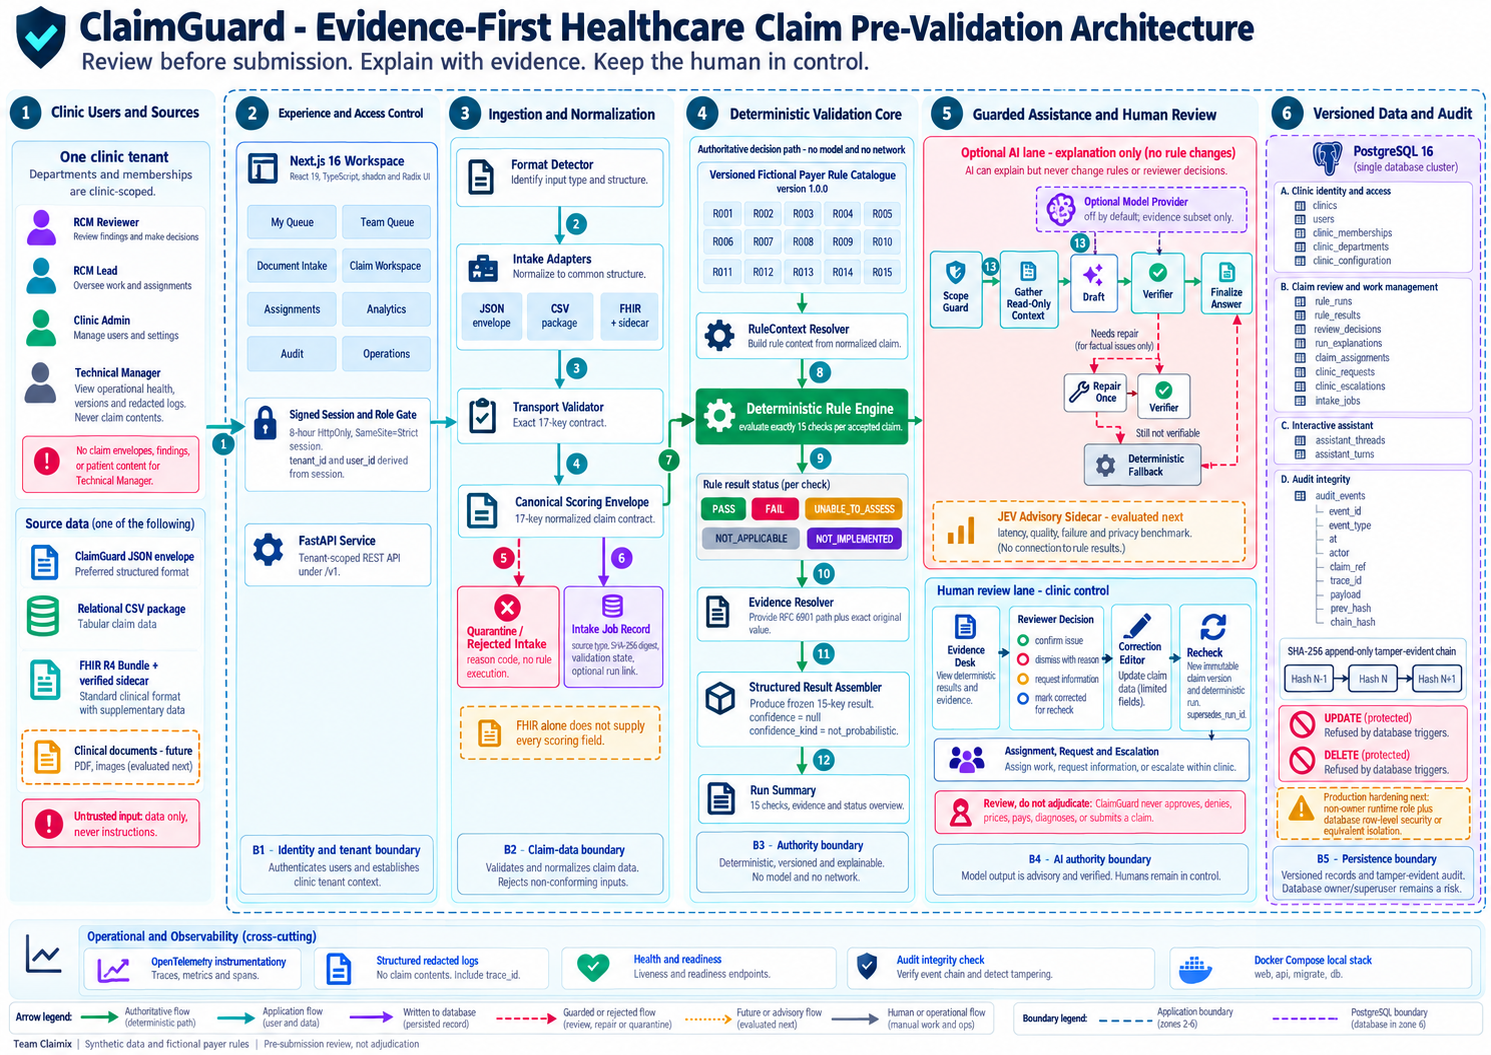
\includegraphics[width=1.03\linewidth,height=0.99\textheight,keepaspectratio]{assets/claimguard-master-architecture.png}}
\captionof{figure}{Global ClaimGuard source architecture. The plate is intentionally presented on a full landscape page to keep labels and trust boundaries readable.}
\label{fig:global-architecture}
\end{center}
\end{landscape}

\chapter{Global Source Architecture}

Figure \ref{fig:global-architecture} organizes the platform into six runtime zones and one cross-cutting operational rail. The central green path is authoritative. Teal links represent application requests. Violet links represent persisted records. Rose links identify guarded, rejected, or security-sensitive behavior. Amber indicates future or advisory work.

\section{Layer 1: clinic users and sources}
One clinic is one tenant. An RCM Reviewer works assigned or self-submitted claims. An RCM Lead also manages assignments and escalations. A Clinic Admin manages the clinic directory, departments, access, routing, analytics, and audit views. A Technical Manager receives operational metadata but is blocked from claim envelopes and findings.

The supported structured sources are a complete ClaimGuard JSON envelope, a relational CSV package, and a FHIR R4 Bundle accompanied by a verified sidecar \cite{fhir-r4}. The sidecar is required because the current educational FHIR projection does not carry every leaf required by the scoring contract. General clinical documents are shown in amber because extraction from PDFs, images, invoices, or narrative reports remains a future proof of concept.

\begin{figure}[H]
\centering
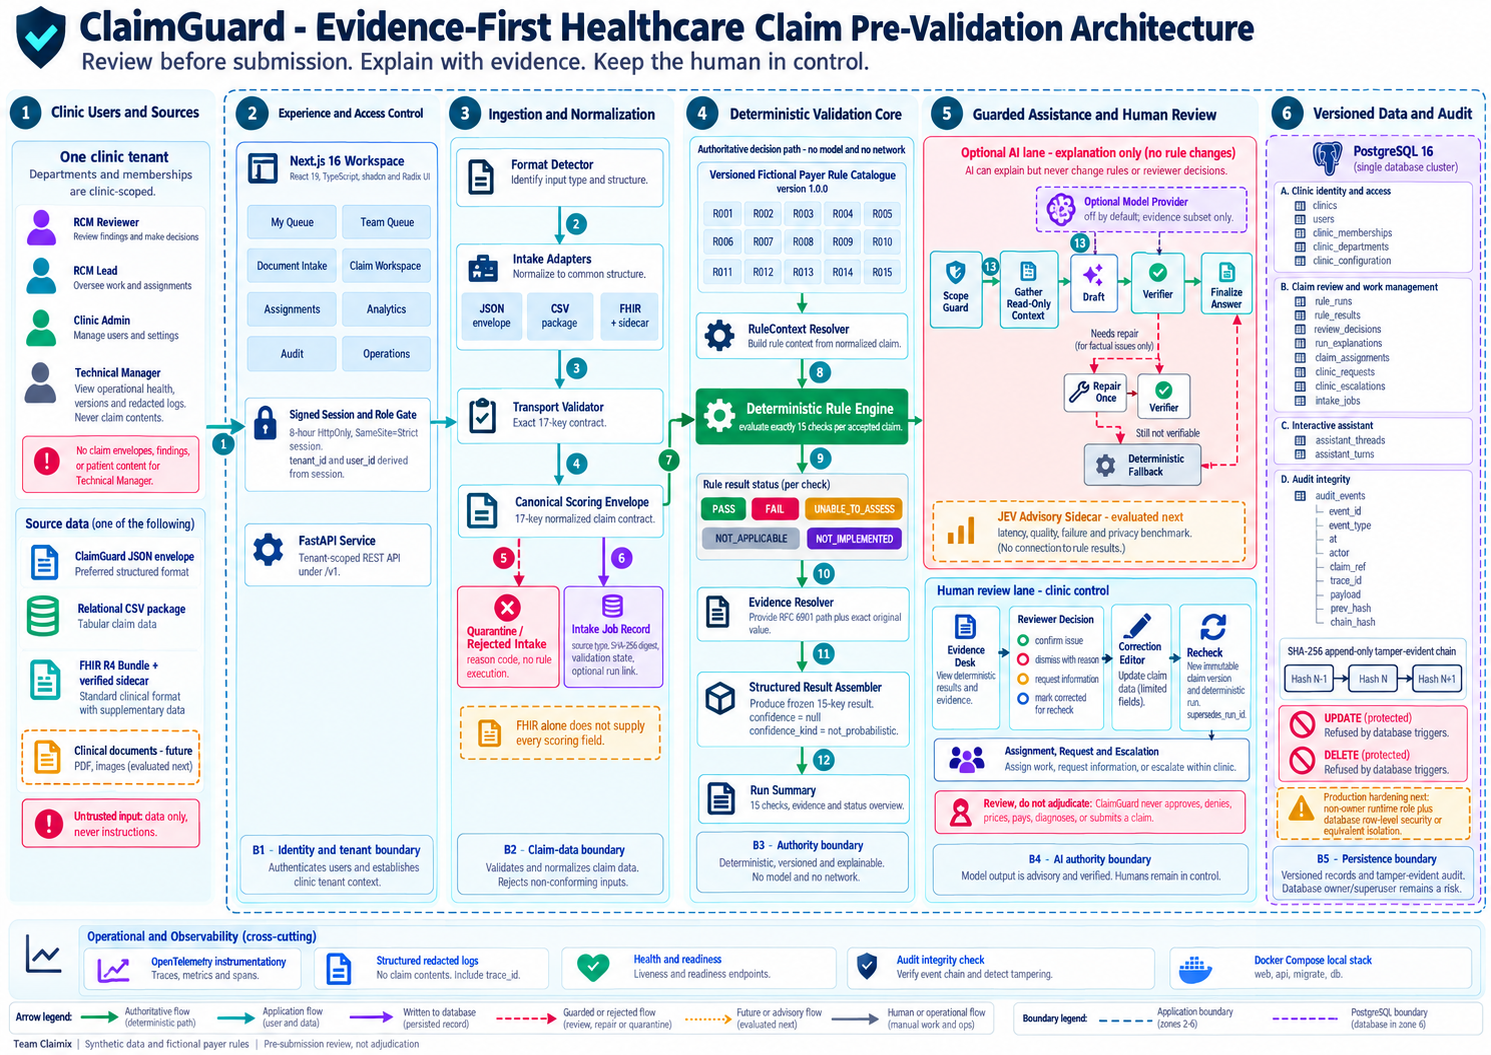
\includegraphics[height=0.66\textheight,trim=0 140 1040 85,clip]{assets/claimguard-master-architecture.png}
\caption{Enlarged view of the clinic roles, supported sources, workspace, and access-control boundary.}
\end{figure}

\section{Layer 2: experience and access control}
The Next.js workspace is the primary product surface. It exposes different navigation and actions according to role, but every protected request still passes through the FastAPI session gate. The session is HMAC-signed, HttpOnly, SameSite Strict, and limited to eight hours. Membership is resolved from current database state, so revoking a membership prevents later access.

The API derives \texttt{tenant\_id} and \texttt{user\_id} from the session rather than trusting request data. This prevents a caller from changing a tenant identifier in a body or query to cross clinic boundaries. The current implementation still relies on application-level tenant predicates. A non-owner runtime database role and row-level security or an equivalent isolation mechanism remain production gates \cite{owasp-authz}.

\section{Layer 3: ingestion and normalization}
The format detector classifies the package before parsing it. It does not guess when a payload is incomplete. JSON, CSV, and FHIR plus sidecar then use dedicated adapters to produce the same candidate envelope. The transport validator checks the exact keys and types. A valid candidate becomes the canonical scoring envelope; an invalid one enters quarantine with a structured reason and does not reach any rule.

An intake job records the source type, SHA-256 source digest, state, validation information, and optional run link. The source digest supports provenance without claiming that the current intake pilot is a general-purpose clinical document archive.

\begin{figure}[H]
\centering
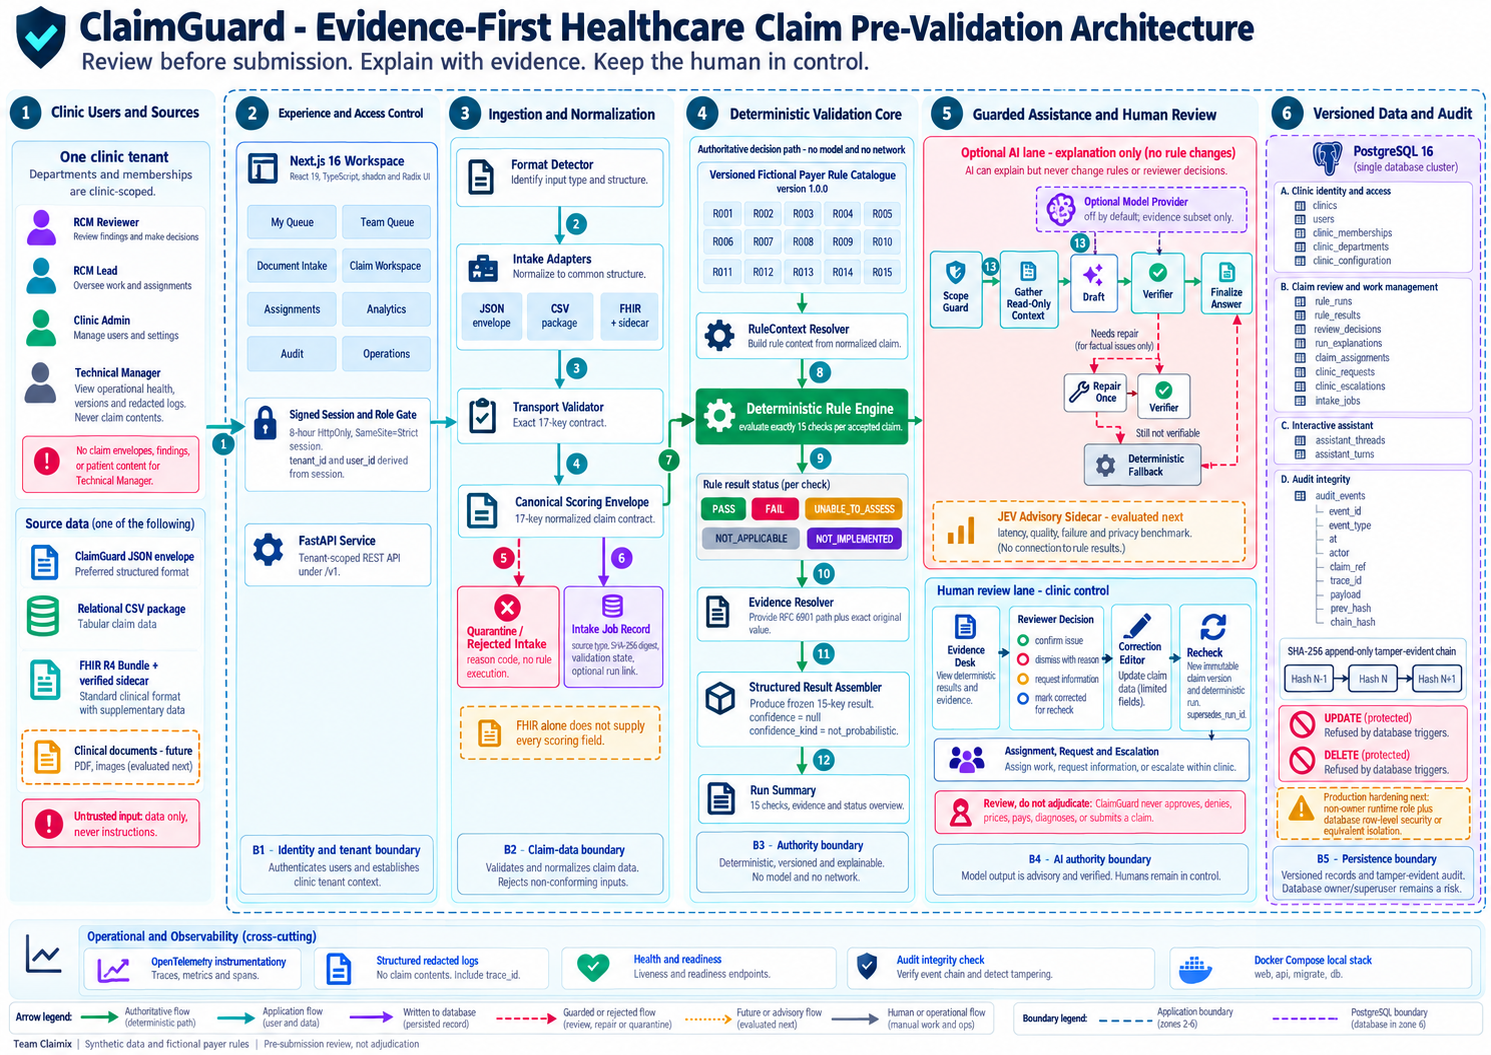
\includegraphics[height=0.68\textheight,trim=445 140 810 85,clip]{assets/claimguard-master-architecture.png}
\caption{Ingestion and normalization layer. Every accepted source converges on the 17-key scoring envelope.}
\end{figure}

\section{Layer 4: deterministic validation core}
The rule catalogue provides rule metadata and fictional policy context. The RuleContext resolver binds the normalized claim to versioned policies, service codes, provider lists, diagnosis catalogues, authorization conditions, required documents, limits, and submission windows. An unknown policy is not replaced with a default.

The engine evaluates R001 to R015 and always emits one result per rule. It distinguishes PASS, FAIL, UNABLE TO ASSESS, NOT APPLICABLE, and NOT IMPLEMENTED. A proven violation takes precedence over missing evidence, while missing evidence prevents an unjustified pass. The evidence resolver then records a pointer and the exact original value that supported the outcome. The result assembler creates the frozen structured record.

\begin{figure}[H]
\centering
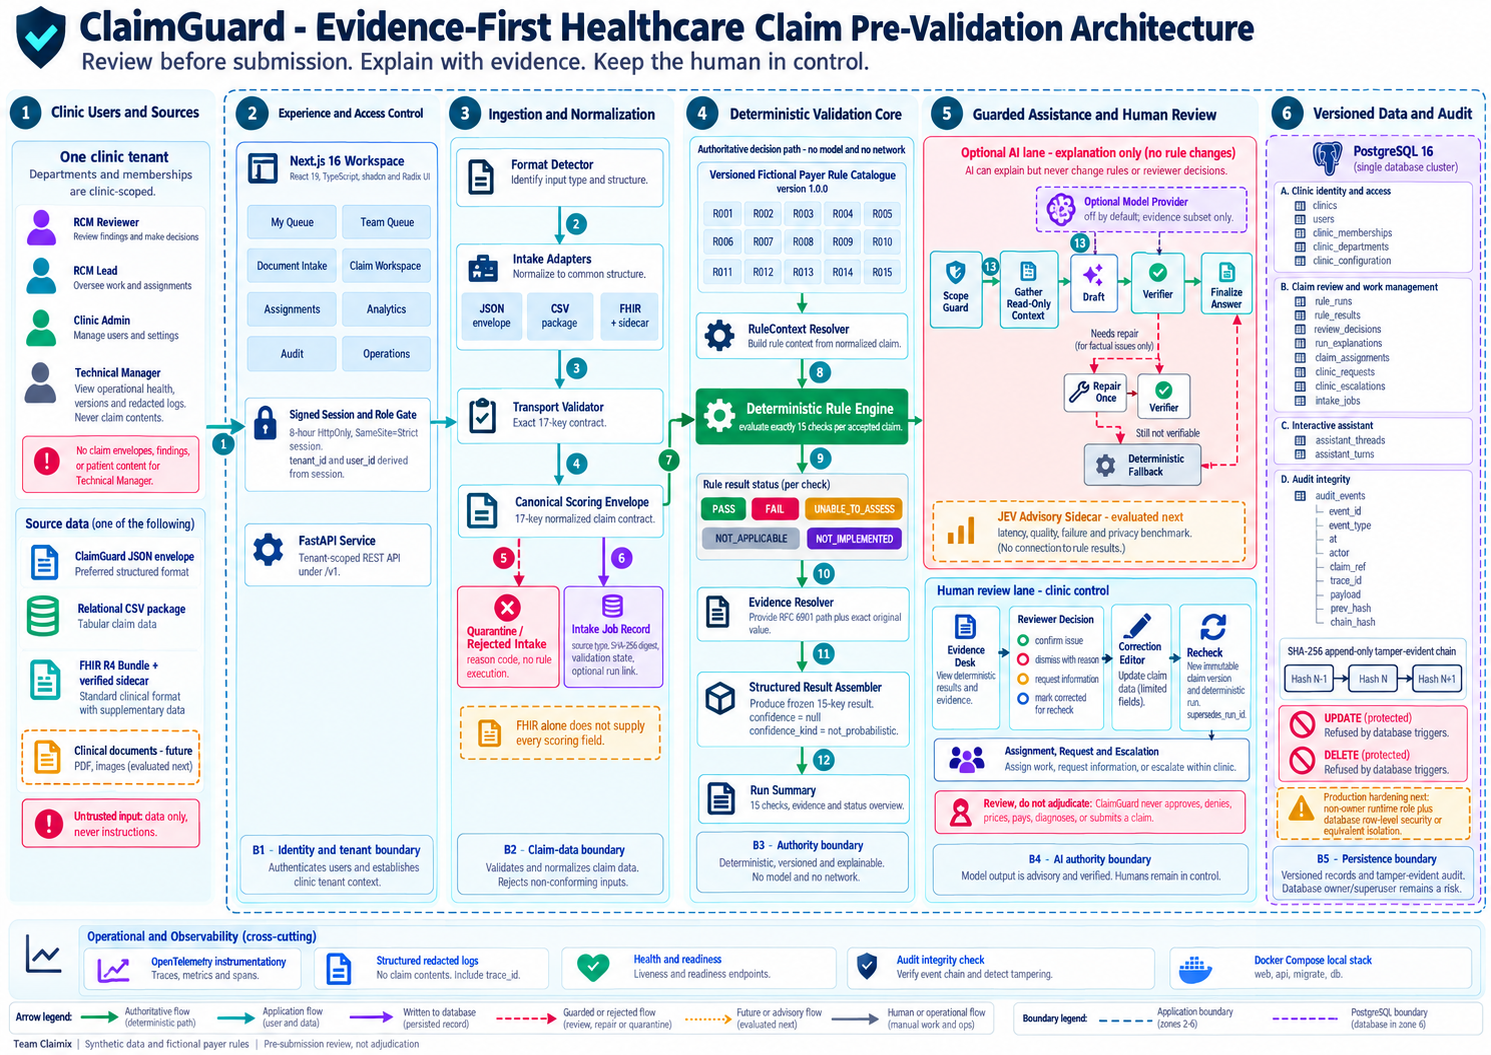
\includegraphics[height=0.69\textheight,trim=680 140 570 85,clip]{assets/claimguard-master-architecture.png}
\caption{Authoritative validation core. No model and no external network are required to establish a result.}
\end{figure}

\section{Layer 5: guarded assistance and human review}
The upper lane is an optional explanation path. A deterministic scope guard runs before any model is reachable. It accepts only questions grounded in the active finding and refuses decision requests, clinical advice, injection attempts, and unrelated questions. The gather step reads the finding, cited evidence values, rule text, relevant policy limits, and the existing conversation. Drafting is optional. The verifier checks the exact answer schema, re-resolves citations, enforces allowed rule identifiers, and rejects prohibited assertions. One repair is allowed; otherwise deterministic fallback text is served.

The lower lane is the accountable workflow. The Evidence Desk aligns the finding with original values and guidance. The reviewer may confirm an issue, dismiss it with a reason, request information, or mark it corrected for recheck. A correction editor changes a limited set of fields under human control. Recheck creates a later immutable version and sends it through the same deterministic path.

\begin{figure}[H]
\centering
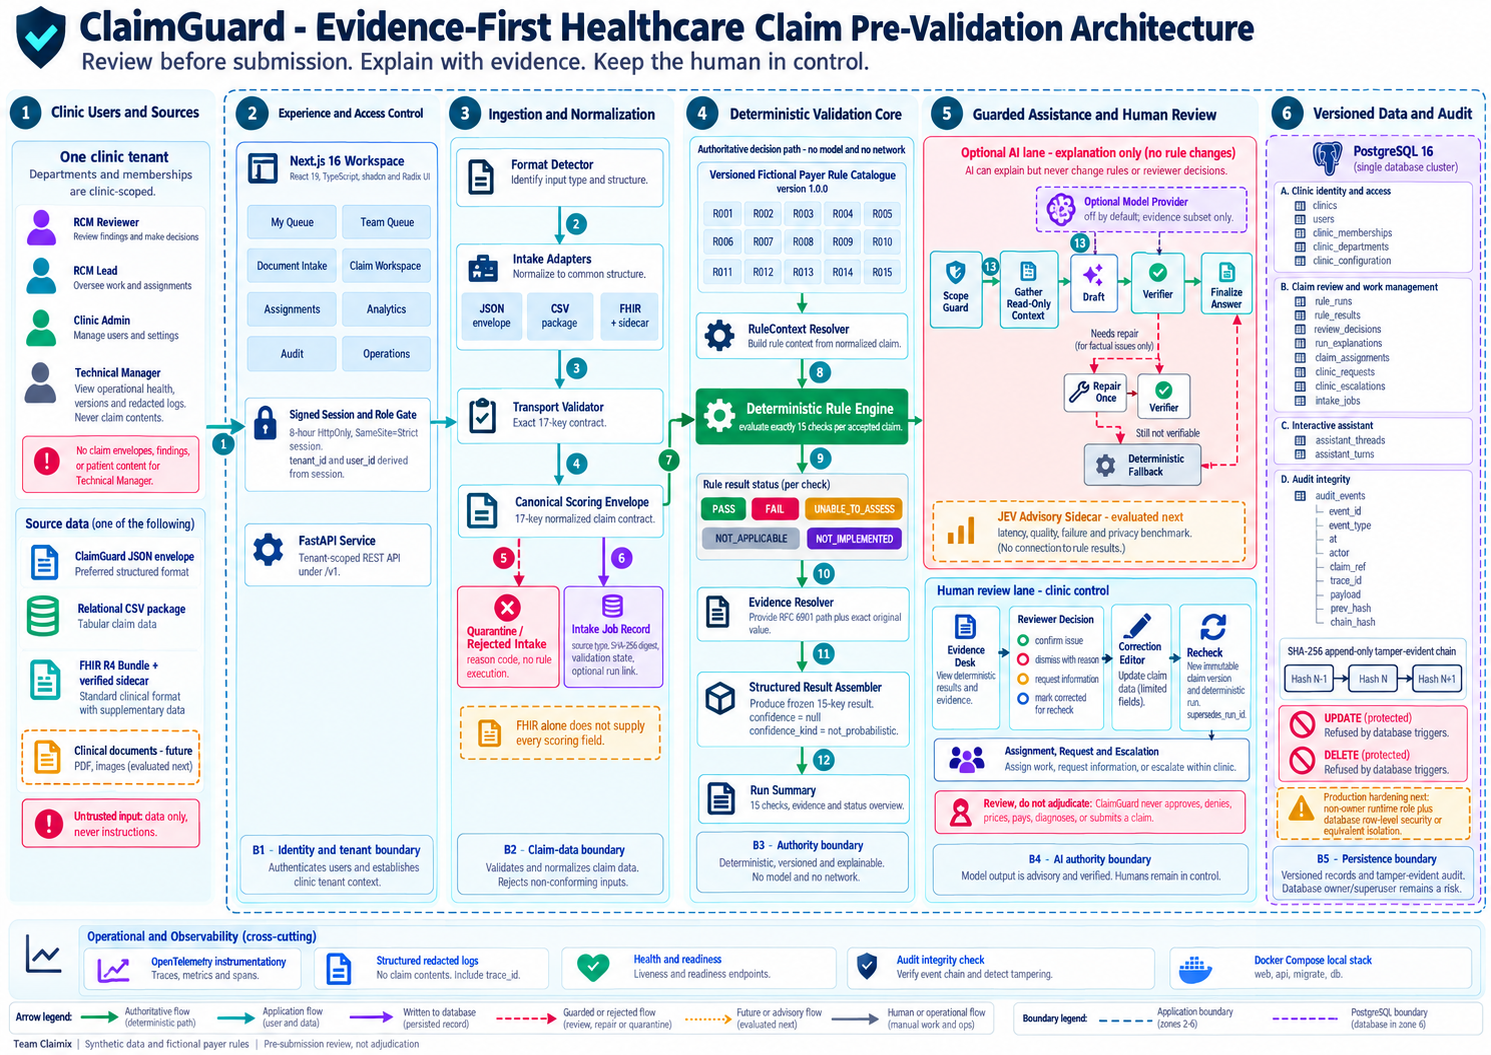
\includegraphics[height=0.68\textheight,trim=915 140 235 85,clip]{assets/claimguard-master-architecture.png}
\caption{Guarded assistance and human review. The model path and reviewer authority remain separate.}
\end{figure}

\section{Layer 6: versioned data, audit, and operations}
PostgreSQL stores the clinic directory, review workflow, explanation provenance, assistant conversations, and audit ledger. The protected tables favor append-only or immutable behavior. The audit chain links each event hash to its predecessor so later modification becomes detectable. The design is tamper-evident, not deletion-proof against a database owner or superuser.

The cross-cutting operational rail includes OpenTelemetry instrumentation \cite{otel-spec}, structured redacted logs, health and readiness checks, audit-integrity verification, and the Docker Compose local stack. Grafana or another monitoring interface is a planned integration, not a component claimed as deployed.

\begin{figure}[H]
\centering
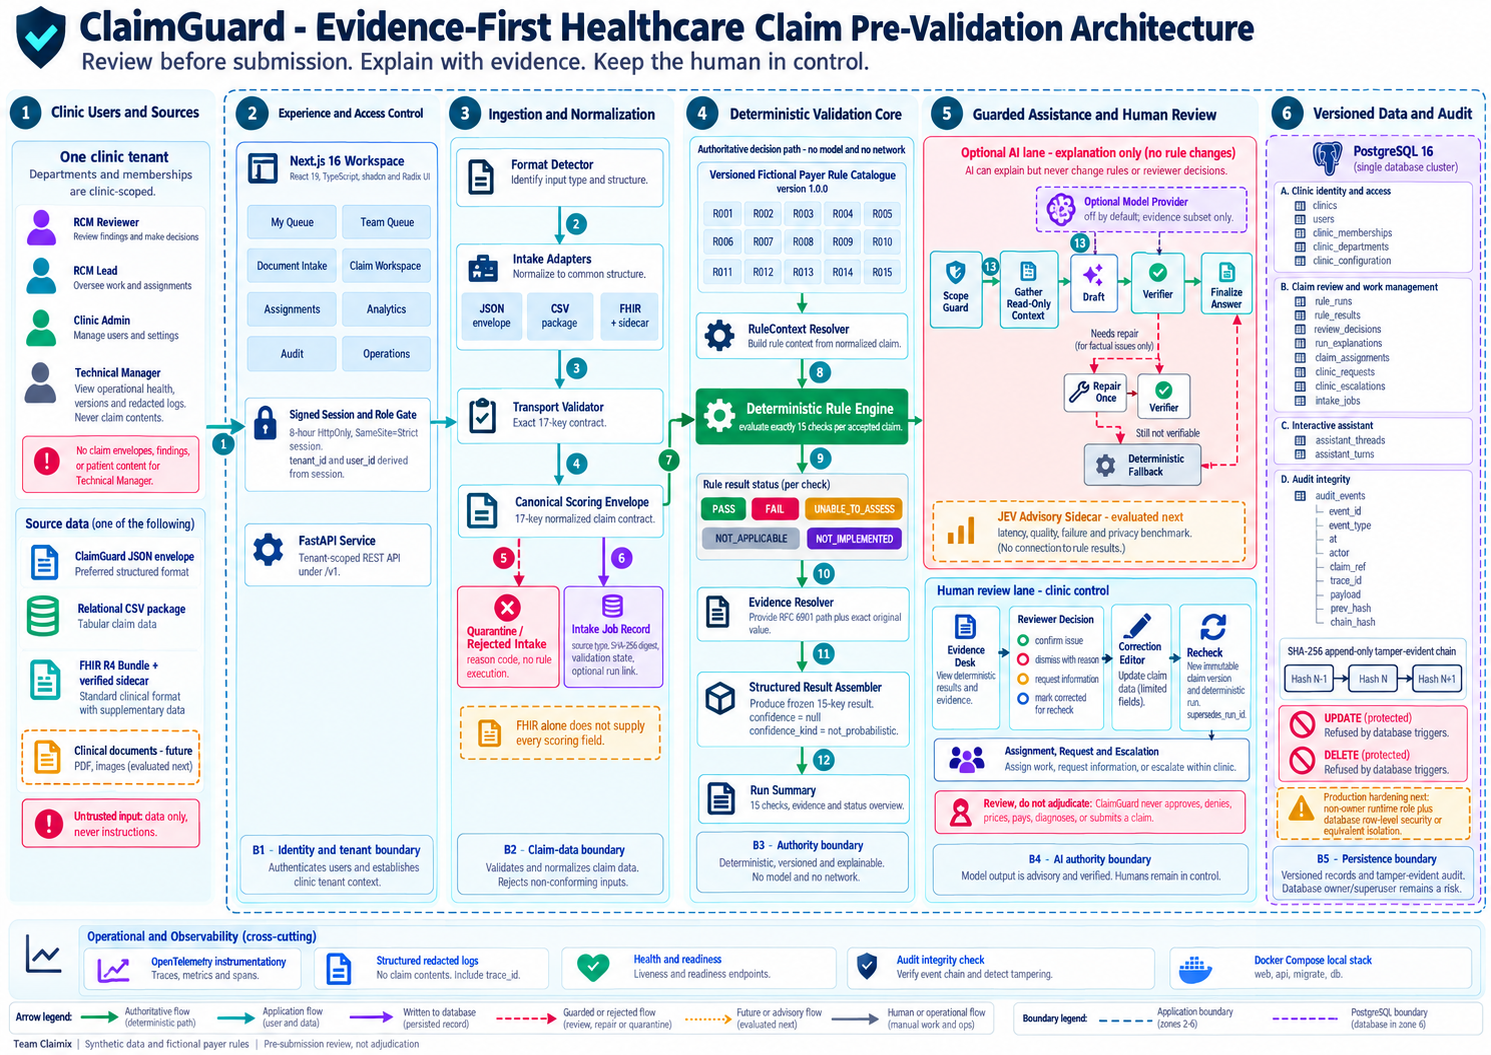
\includegraphics[height=0.69\textheight,trim=1260 140 0 85,clip]{assets/claimguard-master-architecture.png}
\caption{Versioned storage and audit boundary. Review records are tenant-owned and history-preserving.}
\end{figure}

\chapter{Ingestion and Data Flow}

\section{The normalized claim contract}
The scoring envelope contains exactly seventeen top-level keys. These keys cover schema identity, claim and invoice identifiers, patient and member identifiers, provider and payer identifiers, policy and diagnosis identifiers, submission date, currency, total amount, coverage, claim lines, authorizations, attachments, and notes. Nested structures retain the fields needed by the fictional rule catalogue.

Normalization does not mean filling gaps with plausible data. It means mapping known values into a stable structure and reporting unsupported or missing values. This distinction is essential for FHIR. The current mapping recovers a defined subset of envelope paths from the Bundle. The verified sidecar supplies the remaining scoring fields and is compared against every projected path before the package is accepted.

\begin{landscape}
\thispagestyle{plain}
\begin{center}
\vspace*{-14mm}
\makebox[\linewidth][c]{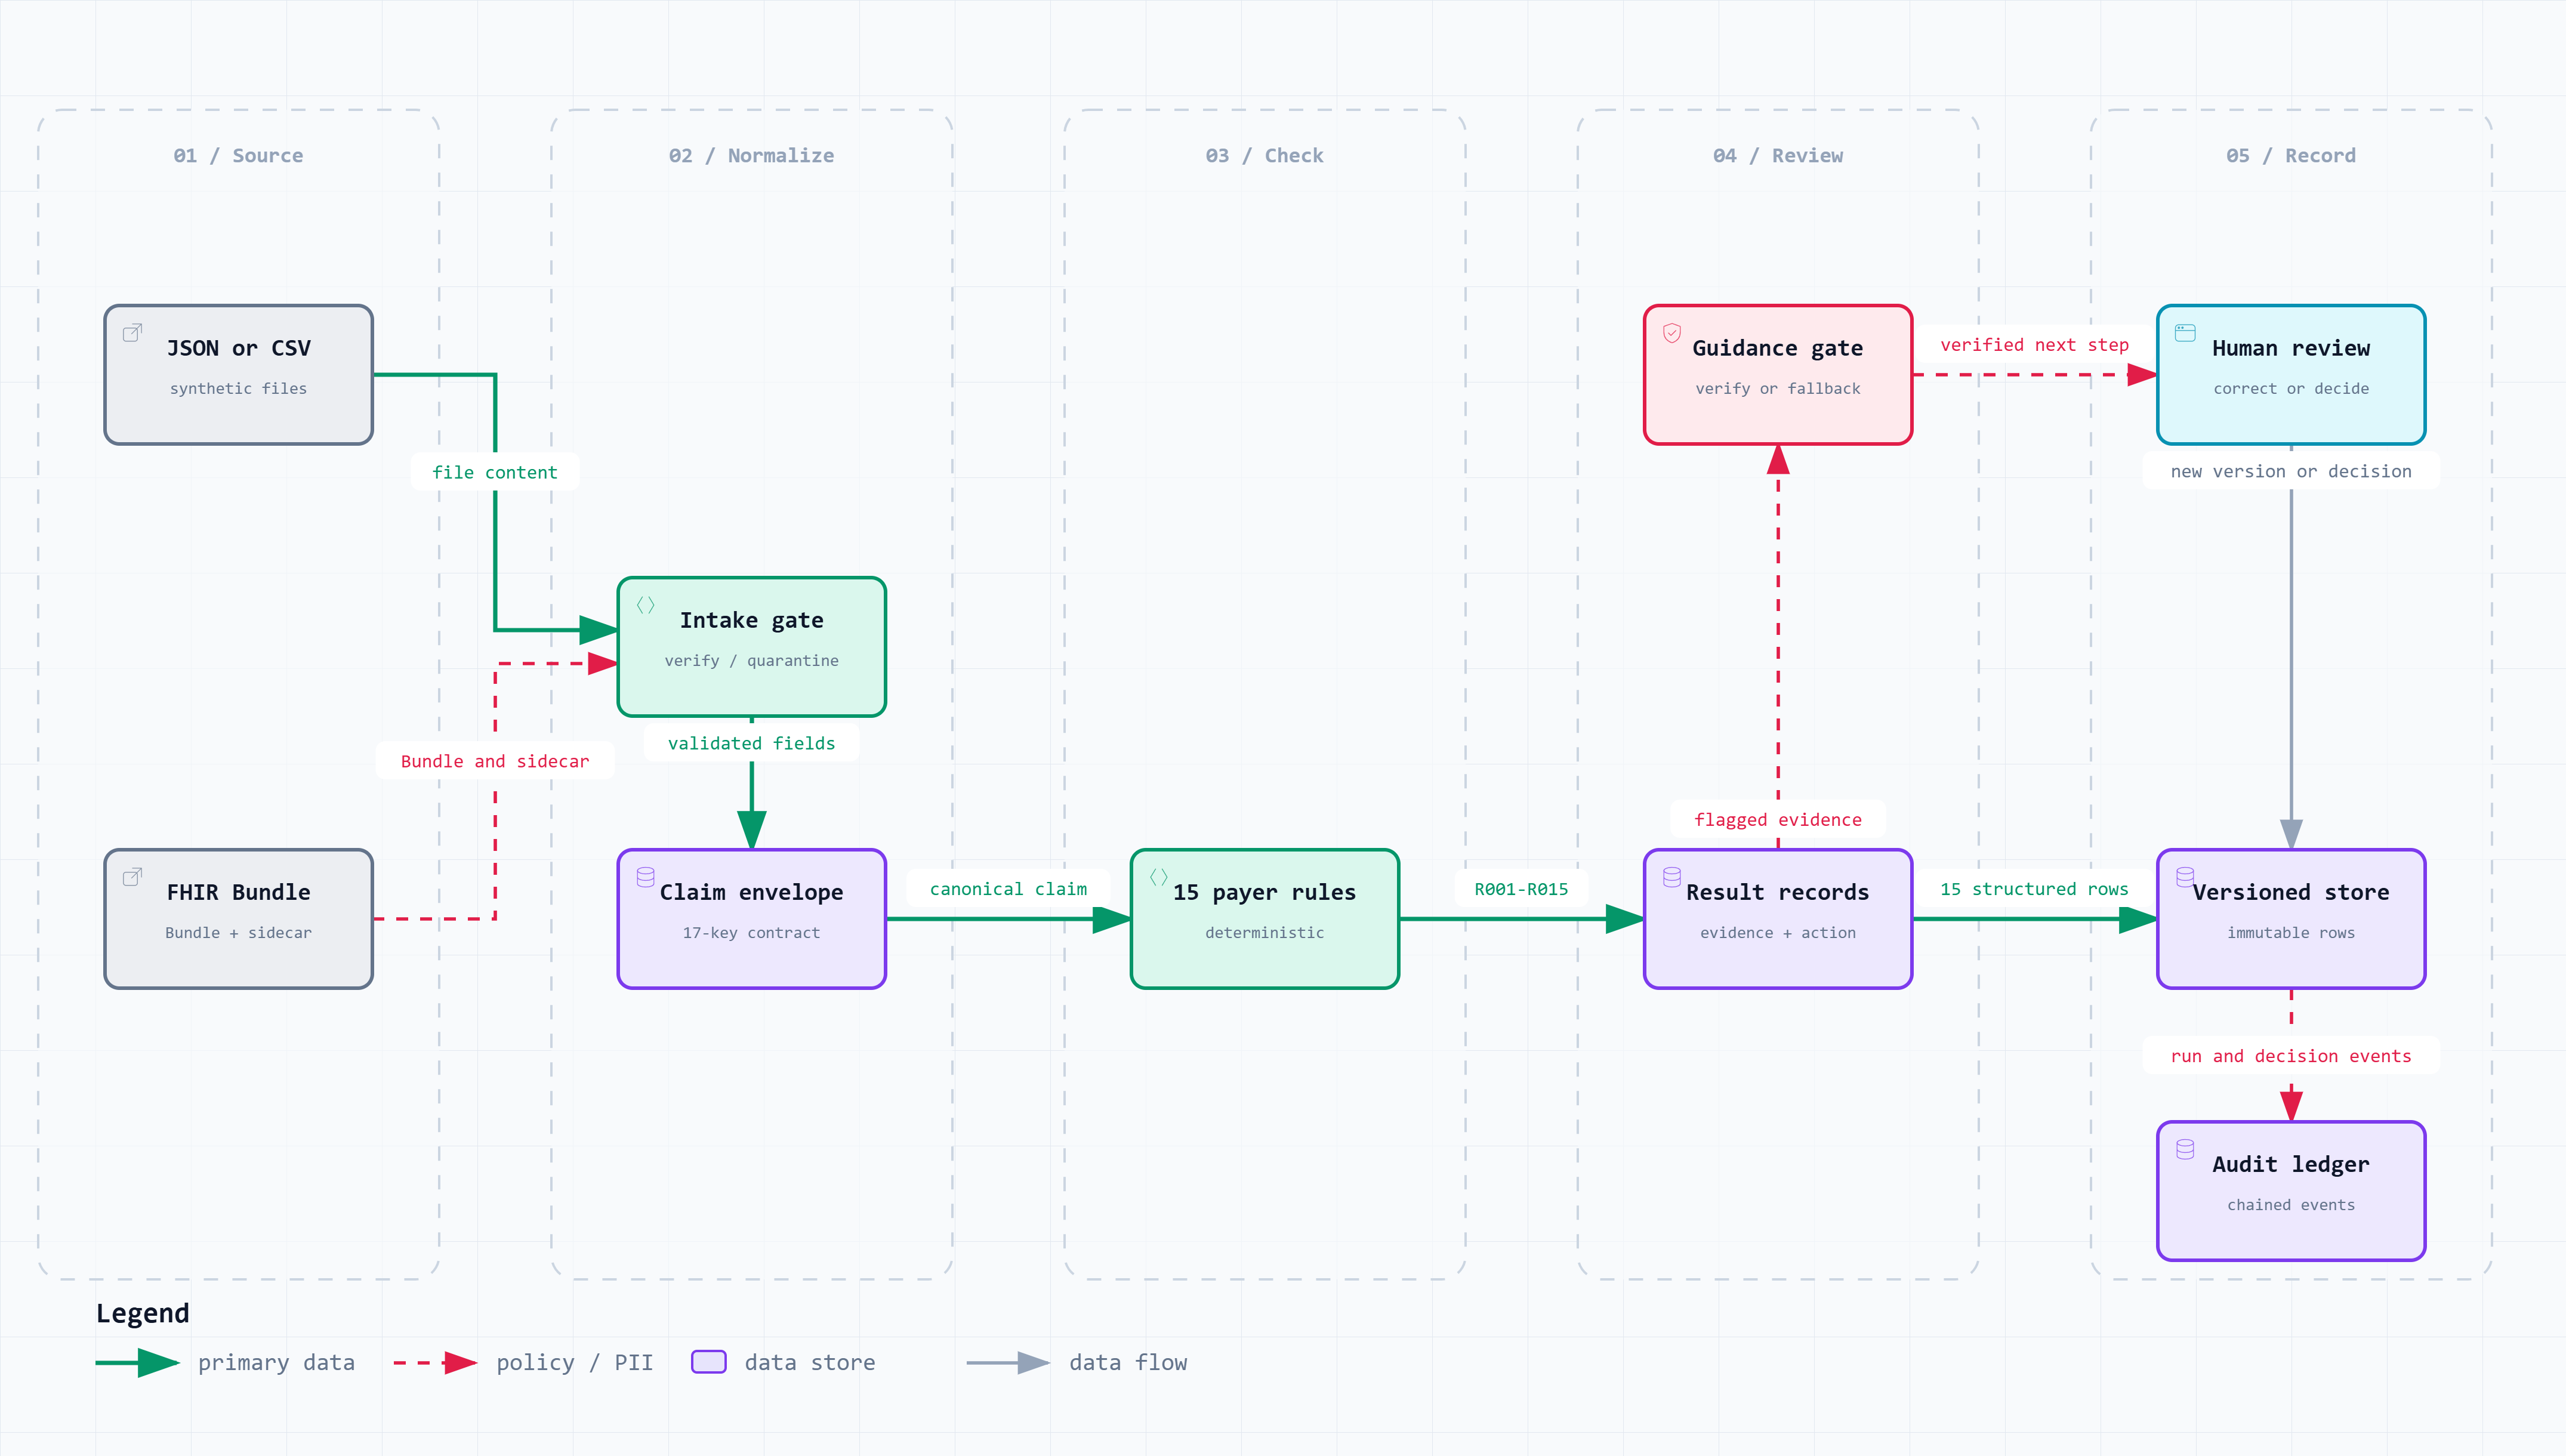
\includegraphics[width=1.08\linewidth]{assets/claim-data-flow.png}}
\captionof{figure}{Claim package data flow from source through normalization, deterministic checks, review, versioning, and the audit ledger.}
\label{fig:dataflow}
\end{center}
\end{landscape}

\section{Flow interpretation}
Figure \ref{fig:dataflow} begins with a synthetic JSON or CSV package, or a FHIR Bundle accompanied by its sidecar. The intake gate validates rather than repairs. The canonical envelope becomes the only object evaluated by the rule engine. Exactly fifteen structured result rows are produced. Findings with attention-worthy outcomes can request a verified explanation, after which a human reviewer decides or corrects. Persisted versions and chained events complete the flow.

The red dashed paths in the figure do not represent a second decision system. They represent policy-sensitive or guarded information movement: the FHIR sidecar supplies missing contract fields, finding evidence constrains the explanation, and run and decision events enter the integrity chain.

\section{Failure behavior}
Malformed JSON, missing envelope keys, inconsistent FHIR sidecar values, invalid types, and unsupported shapes do not reach the engine. The API or batch process returns a structured ingestion error and records the failed intake where appropriate. This behavior prevents a parser defect from becoming a silent pass and keeps the reviewer informed about whether the system rejected a package or evaluated it.

\chapter{Deterministic Rules and Structured Explainability}

\section{Rule catalogue}
The fifteen fictional payer rules cover completeness, chronology, eligibility context, provider and member consistency, duplicate detection, arithmetic, authorization, documentation, service support, policy limits, submission windows, and currency. Table \ref{tab:rules} summarizes their intent.

\begin{longtable}{>{\bfseries}p{14mm} p{42mm} p{85mm}}
\caption{Fictional payer rules evaluated for every accepted claim.}\label{tab:rules}\\
\toprule
\textbf{Rule} & \textbf{Check} & \textbf{Question answered}\\
\midrule
\endfirsthead
\toprule
\textbf{Rule} & \textbf{Check} & \textbf{Question answered}\\
\midrule
\endhead
R001 & Required information & Are the mandatory claim and identity fields present?\\
R002 & Chronology & Are service, coverage, authorization, and submission dates logically ordered?\\
R003 & Active coverage & Was coverage active on the relevant service date?\\
R004 & Member consistency & Do the member, beneficiary, and patient references agree?\\
R005 & Provider network & Is the provider supported by the selected fictional policy?\\
R006 & Possible duplicate & Do two lines represent a suspicious duplicate service entry?\\
R007 & Line arithmetic & Does quantity multiplied by unit price agree with the line amount?\\
R008 & Authorization reference & Does a service that requires authorization cite one?\\
R009 & Authorization match & Does the authorization match patient, service, date, status, and limits?\\
R010 & Supporting document & Is the required document present and in an acceptable state?\\
R011 & Service catalogue & Is the service code supported by the fictional catalogue?\\
R012 & Claim total & Does the total agree with the sum of line amounts?\\
R013 & Quantity and price limits & Are line quantity and price within fictional policy limits?\\
R014 & Submission window & Was the claim submitted within the policy's allowed number of days?\\
R015 & Currency & Does the claim currency match the policy currency?\\
\bottomrule
\end{longtable}

\section{Five-state semantics}
PASS means that the available evidence does not violate that fictional rule. FAIL means a violation is demonstrated. UNABLE TO ASSESS means required evidence is missing or insufficient. NOT APPLICABLE means the rule does not apply to the claim. NOT IMPLEMENTED is a distinct state that prevents unfinished logic from being presented as a pass.

Confidence is not invented for deterministic rules. The result uses a null confidence value and the explicit kind \texttt{not\_probabilistic}. This is more truthful than assigning a number such as 1.0 to deterministic code and later treating it as calibrated probability.

\section{Structured result record}
Each result has fifteen fixed keys: claim identity, rule identity and version, status, severity, affected line identifiers, evidence, rule source, explanation, corrective action, confidence, confidence kind, human-review requirement, method, and review status. The scorer rejects missing or additional keys, unknown status values, incorrect rule version or source, and evidence whose stored value cannot be re-resolved from the submitted envelope.

This strictness improves the product interface. The UI does not need to infer which object belongs to which rule or whether a recommendation can be linked to a source. The same contract supports machine evaluation, reviewer display, persistence, replay, and later analysis.

\section{Explanation and correction recommendation}
The deterministic finding answers what happened. The assistance layer helps answer why the issue matters and what the reviewer should inspect next. Its output uses a small exact schema containing the explanation, correction recommendation, cited evidence paths, cited rule identifiers, and a human-review flag.

The verifier rejects fabricated evidence, foreign rule identifiers, unsupported adjudication or clinical claims, and instruction-shaped text. When the model is disabled or its output fails, deterministic wording remains available and the provenance says that fallback occurred. The reviewer can therefore distinguish accepted model wording from a safe twin.

\chapter{Reviewer Lifecycle and AI Controls}

\section{One claim over time}
The global architecture shows ownership, while a sequence diagram shows time. Figure \ref{fig:sequence} follows an accepted package through tenant authorization, rule evaluation, optional assistance, persistence, review, and correction. The database write stores the run, fifteen results, provenance, and event as one review record. A later decision appends rather than replacing the result.

\begin{landscape}
\thispagestyle{plain}
\begin{center}
\vspace*{-14mm}
\makebox[\linewidth][c]{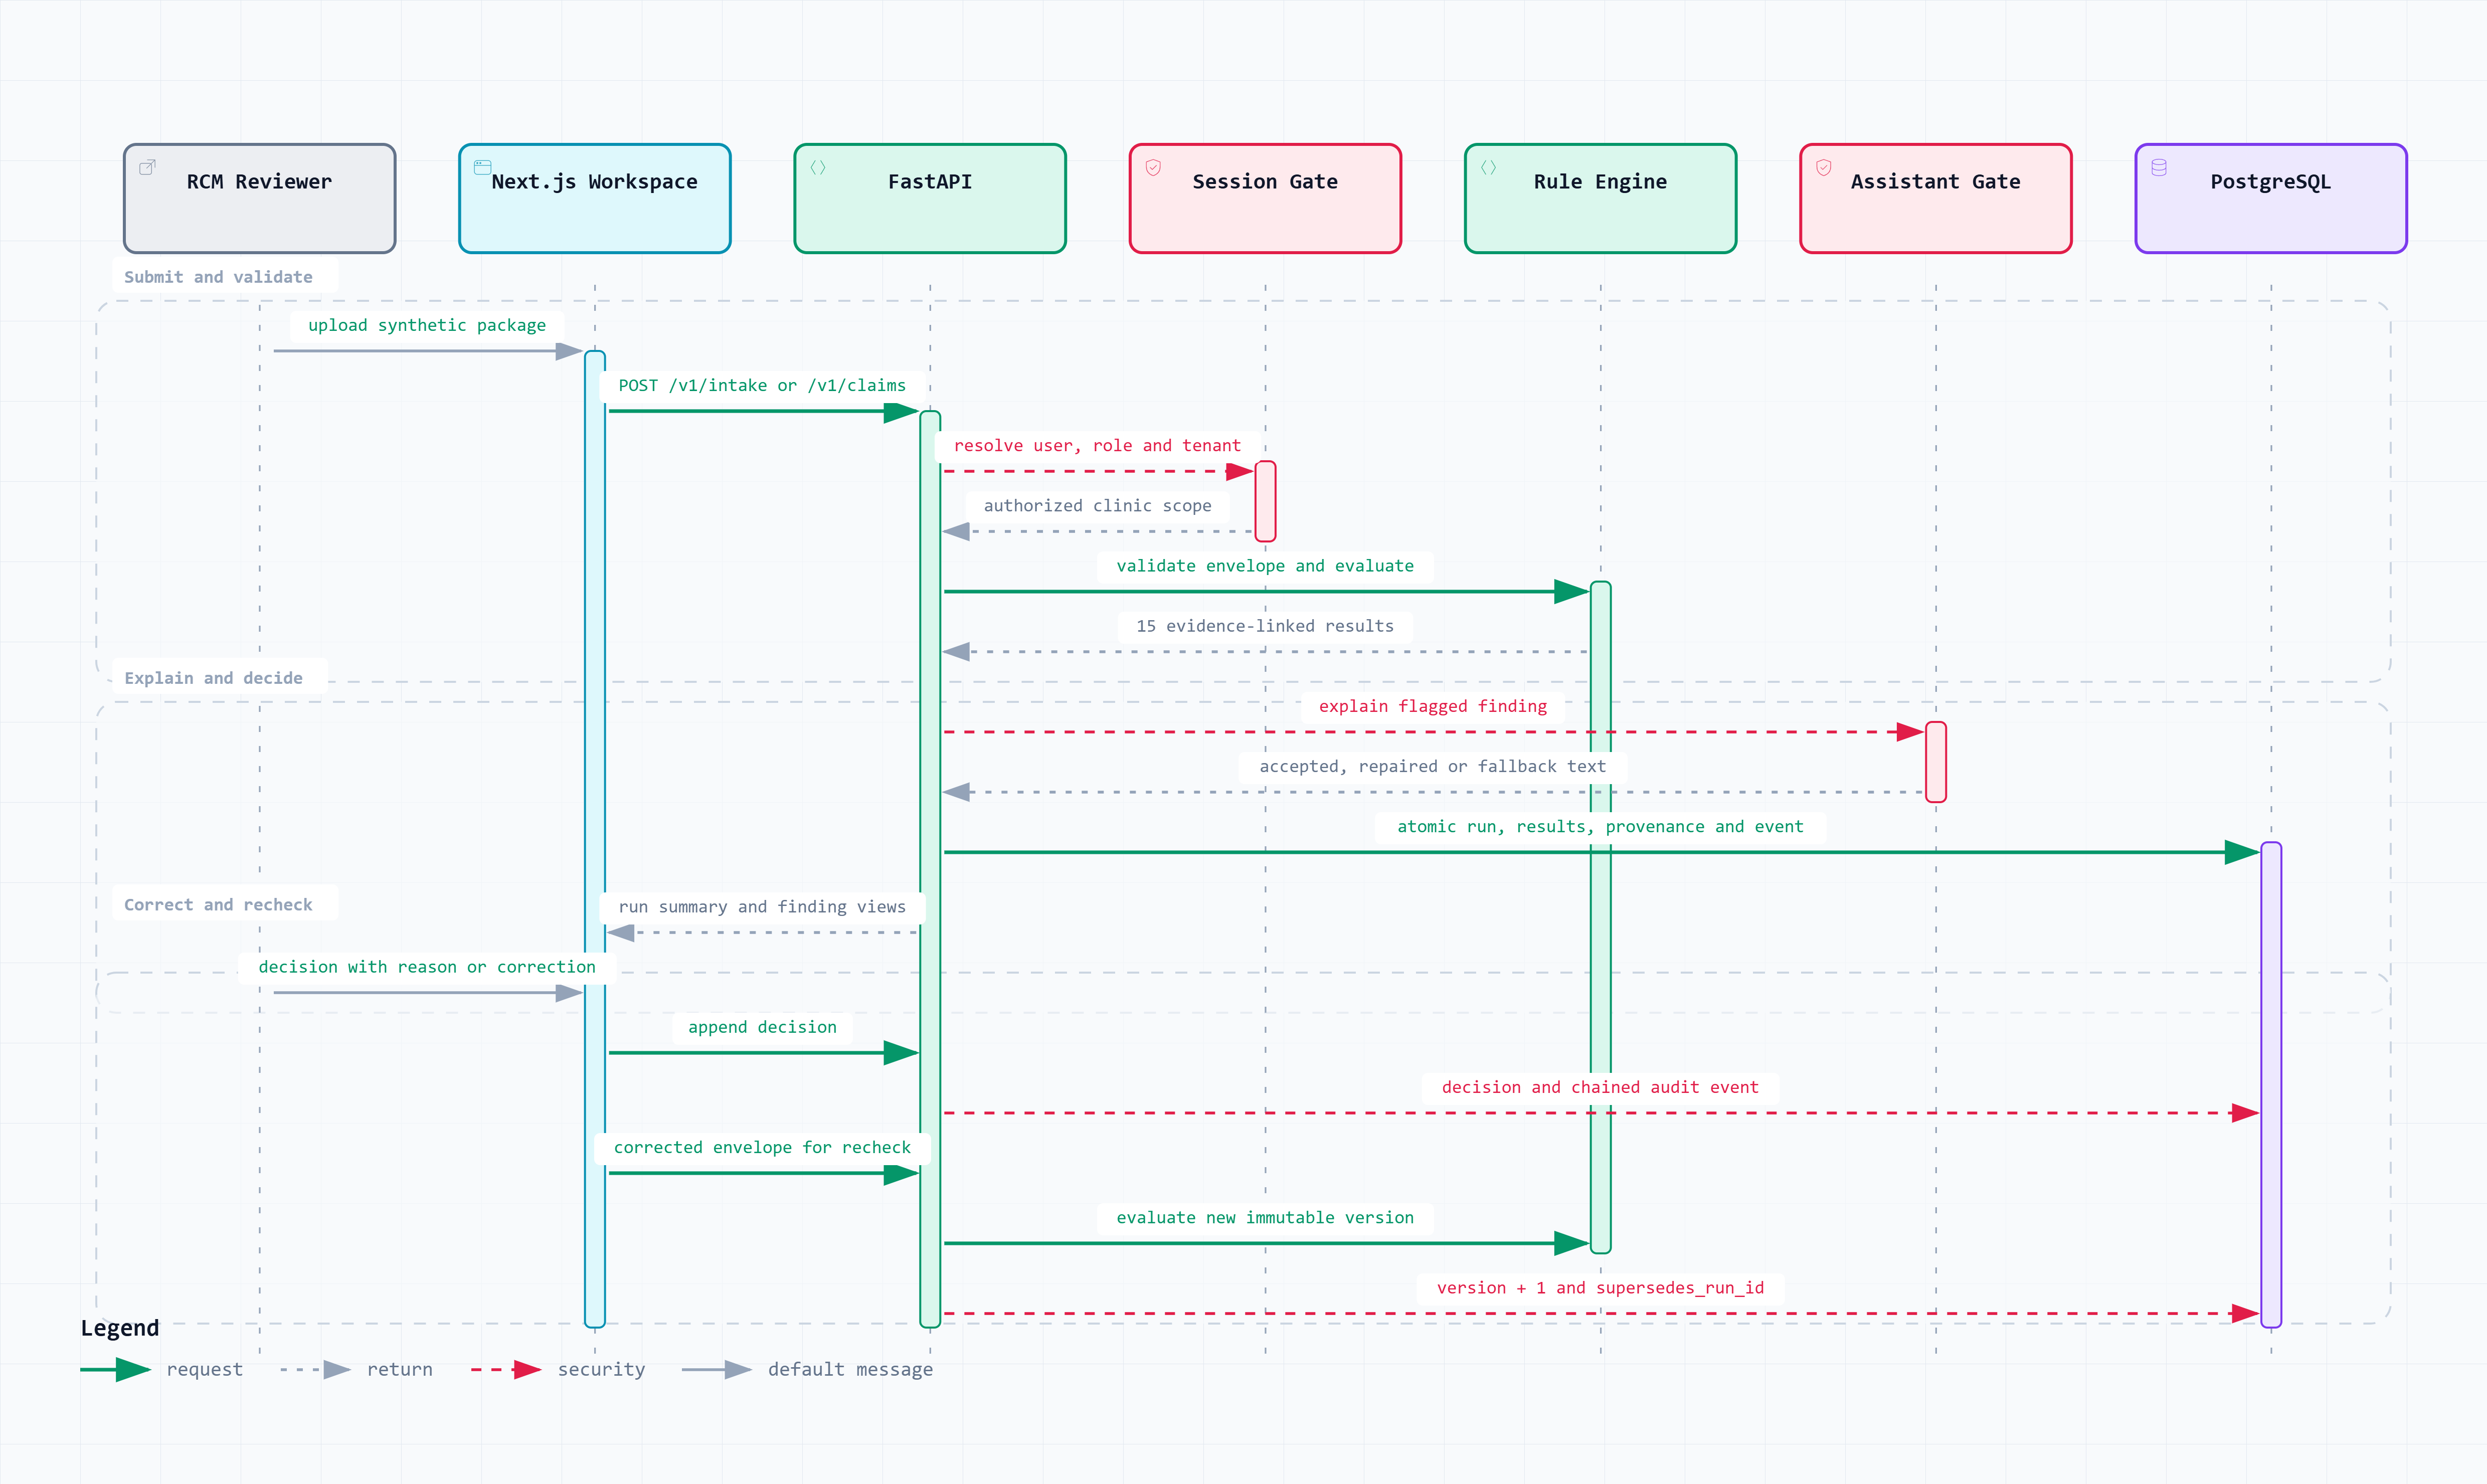
\includegraphics[width=1.03\linewidth]{assets/reviewer-lifecycle.png}}
\captionof{figure}{Sequence of claim submission, guarded explanation, reviewer decision, correction, and versioned recheck.}
\label{fig:sequence}
\end{center}
\end{landscape}

\section{The interactive assistant as a bounded graph}
The assistant is not a free-running agent. It follows a fixed graph in which only drafting and one repair may call a model. Every tool before the model is read-only, and every output after the model is verified.

\begin{figure}[H]
\centering
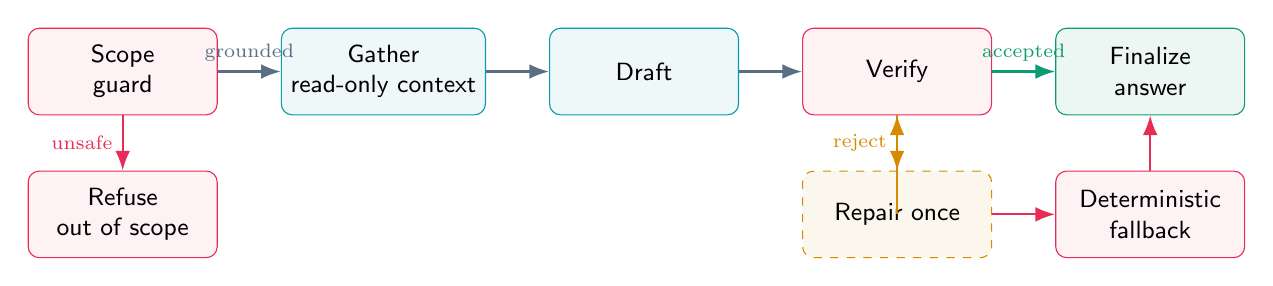
\begin{tikzpicture}[
  node distance=7mm and 8mm,
  box/.style={draw=cgTeal,rounded corners,fill=cgTeal!7,minimum width=24mm,minimum height=11mm,font=\sffamily\small,align=center},
  sec/.style={box,draw=cgRose,fill=cgRose!6},
  ok/.style={box,draw=cgGreen,fill=cgGreen!8},
  future/.style={box,draw=cgAmber,dashed,fill=cgAmber!7},
  flow/.style={-{Latex[length=2.5mm]},thick,cgSlate}
]
  \node[sec] (scope) {Scope\\guard};
  \node[box,right=of scope] (gather) {Gather\\read-only context};
  \node[box,right=of gather] (draft) {Draft};
  \node[sec,right=of draft] (verify) {Verify};
  \node[ok,right=of verify] (final) {Finalize\\answer};
  \node[future,below=of verify] (repair) {Repair once};
  \node[sec,below=of final] (fallback) {Deterministic\\fallback};
  \node[sec,below=of scope] (refuse) {Refuse\\out of scope};
  \draw[flow] (scope) -- node[above,font=\scriptsize]{grounded} (gather);
  \draw[flow] (gather) -- (draft);
  \draw[flow] (draft) -- (verify);
  \draw[flow,cgGreen] (verify) -- node[above,font=\scriptsize]{accepted} (final);
  \draw[flow,cgAmber] (verify) -- node[left,font=\scriptsize]{reject} (repair);
  \draw[flow,cgAmber] (repair) -| (verify);
  \draw[flow,cgRose] (repair) -- (fallback);
  \draw[flow,cgRose] (fallback) -- (final);
  \draw[flow,cgRose] (scope) -- node[left,font=\scriptsize]{unsafe} (refuse);
\end{tikzpicture}
\caption{Bounded assistant control graph. No node writes to the claim result or reviewer decision.}
\end{figure}

\section{Why a small language model still needs this structure}
A smaller model can reduce deployment cost and make self-hosting more practical, but size does not guarantee grounded behavior. Fine-tuning can improve style and domain vocabulary, yet it cannot replace runtime authority controls. ClaimGuard therefore evaluates model candidates on evidence fidelity, correction usefulness, refusal behavior, latency, and consistency. A candidate becomes deployable only when it passes those measurements without weakening deterministic fallback \cite{nist-ai-rmf,owasp-llm}.

The benchmark and fine-tuning work remain separate from the Phase 1 authority path. The current default is model-off. That state is not a broken mode: the same interface serves deterministic explanation and identifies its provenance.

\chapter{Logical Data and Audit Architecture}

\section{Database organization}
Figure \ref{fig:database} groups the PostgreSQL schema by responsibility \cite{postgresql16}. Clinic identity tables establish tenants, users, memberships, departments, and configuration. Review tables preserve intake jobs, rule runs, results, assignments, requests, escalations, decisions, and explanation provenance. Assistant tables are separate so a conversation cannot become a rule result by accident. The audit ledger preserves the event sequence.

\begin{landscape}
\thispagestyle{plain}
\begin{center}
\vspace*{-14mm}
\makebox[\linewidth][c]{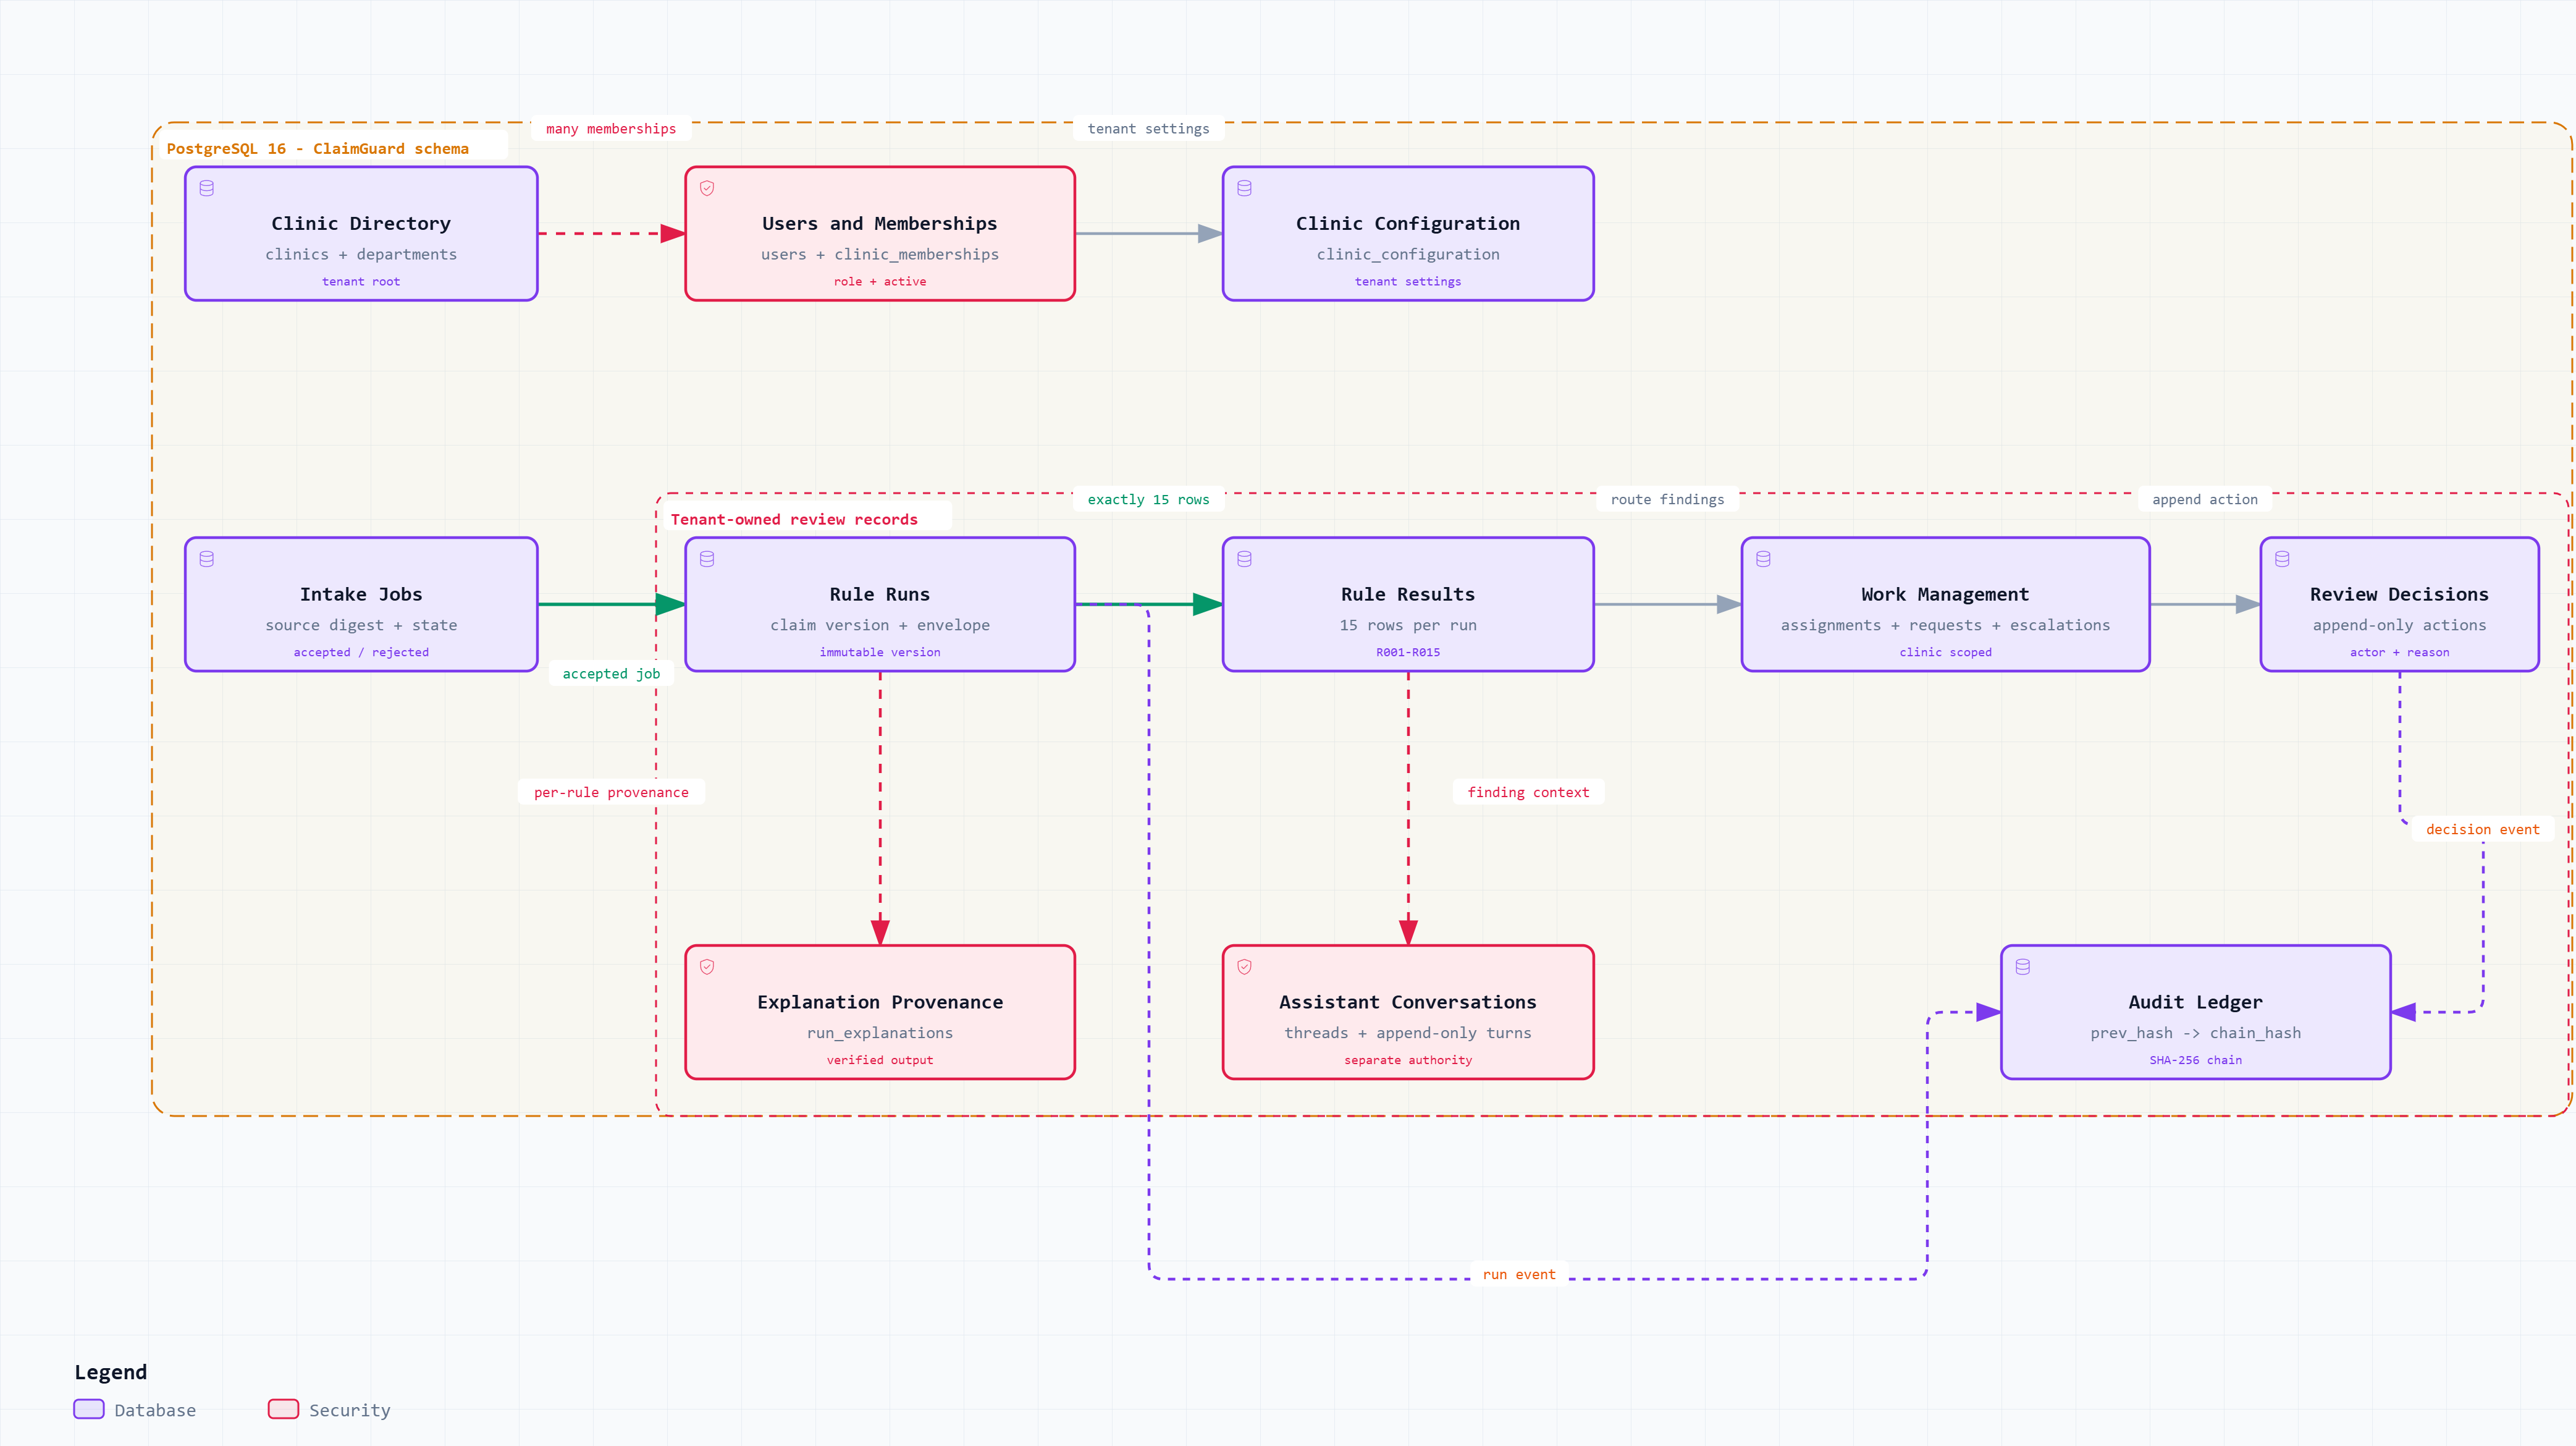
\includegraphics[width=1.08\linewidth]{assets/database-architecture.png}}
\captionof{figure}{Logical PostgreSQL architecture and the principal relationships between tenant, run, result, workflow, assistant, and audit records.}
\label{fig:database}
\end{center}
\end{landscape}

\section{Important cardinalities and invariants}

\begin{table}[H]
\centering
\caption{Principal data relationships.}
\begin{tabularx}{\textwidth}{>{\bfseries}p{42mm} X}
\toprule
Relationship & Invariant\\
\midrule
Clinic to membership & A clinic has many active or revoked memberships; the membership carries the role used by the API.\\
Run to result & Every accepted run has exactly fifteen unique rule results, one for each R001 to R015.\\
Run to decision & A run can have many append-only decision events. Actor and reason are required.\\
Run to explanation provenance & A per-rule record states whether model wording was accepted, repaired, declined, or replaced by fallback.\\
Run to corrected run & The newer run carries the next version and references the earlier run through \texttt{supersedes\_run\_id}.\\
Run and rule to assistant thread & A reviewer owns a conversation for one tenant, run, and rule. Other reviewers receive no existence disclosure.\\
Thread to turn & Turns are append-only, ordered by sequence, and carry model, prompt, verification, latency, and receipt information.\\
Event to previous event & \texttt{prev\_hash} links the event to the previous global ledger digest; \texttt{chain\_hash} commits the current content and link.\\
\bottomrule
\end{tabularx}
\end{table}

\section{Tamper-evident audit chain}
The database trigger computes each event's digest from a canonical serialization of its content and the previous chain hash. In conceptual form:

\[
H_i = \operatorname{SHA256}(H_{i-1} \parallel C_i)
\]

where \(C_i\) is the normalized event content. Verification recomputes the sequence and reports a mismatch if content or linkage has changed. Run creation and reviewer decisions append events in the same transaction as their domain records. This prevents a successful decision write without its corresponding audit event under ordinary operation.

The ledger is accurately described as append-only and tamper-evident for the protected application path. A database owner can still remove triggers, truncate storage, or alter surrounding infrastructure. Production deployment therefore requires restricted ownership, backups, retention controls, off-system verification, and incident response.

\begin{figure}[H]
\centering
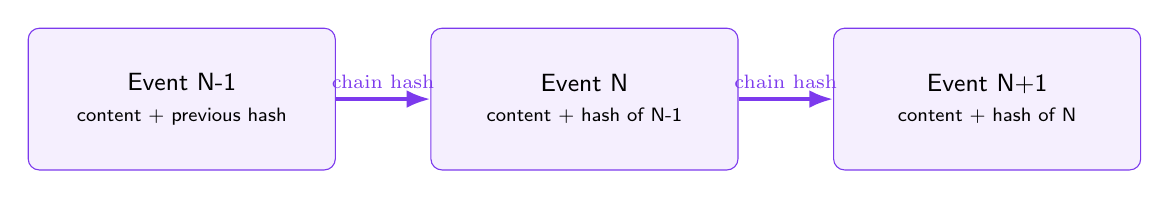
\begin{tikzpicture}[node distance=12mm, every node/.style={font=\sffamily\small}]
  \node[draw=cgViolet,rounded corners,fill=cgViolet!8,minimum width=39mm,minimum height=18mm,align=center] (e1) {Event N-1\\\scriptsize content + previous hash};
  \node[draw=cgViolet,rounded corners,fill=cgViolet!8,right=of e1,minimum width=39mm,minimum height=18mm,align=center] (e2) {Event N\\\scriptsize content + hash of N-1};
  \node[draw=cgViolet,rounded corners,fill=cgViolet!8,right=of e2,minimum width=39mm,minimum height=18mm,align=center] (e3) {Event N+1\\\scriptsize content + hash of N};
  \draw[-{Latex[length=3mm]},line width=1.3pt,cgViolet] (e1) -- node[above,font=\scriptsize]{chain hash} (e2);
  \draw[-{Latex[length=3mm]},line width=1.3pt,cgViolet] (e2) -- node[above,font=\scriptsize]{chain hash} (e3);
\end{tikzpicture}
\caption{Audit events are linked by content-dependent SHA-256 digests.}
\end{figure}

\chapter{Implementation and Verification}

\section{Technology stack}

\begin{table}[H]
\centering
\caption{Primary implementation technologies.}
\begin{tabularx}{\textwidth}{>{\bfseries}p{38mm} p{43mm} X}
\toprule
Layer & Technology & Responsibility\\
\midrule
Frontend & Next.js 16, React 19, TypeScript, shadcn, Radix UI & Role-specific workspaces, intake, evidence-led review, correction, administration, analytics, and operations.\\
API & FastAPI, Pydantic & Tenant-scoped HTTP contracts, session enforcement, orchestration, structured errors, and OpenAPI documentation.\\
Rules & Python, Pydantic, JSON Pointer & Transport validation, versioned policy context, fifteen deterministic rules, evidence resolution, and frozen result records.\\
Assistance & LangGraph-style bounded graph, optional model provider & Scope control, read-only context gathering, drafting, verification, one repair, fallback, and provenance.\\
Persistence & PostgreSQL 16, SQLAlchemy, psycopg, Alembic & Tenant-owned records, versioned runs, append-only decisions, assistant turns, triggers, and audit chain.\\
Operations & Docker Compose, OpenTelemetry, structured logging & Reproducible local stack, health checks, traces, metrics hooks, and redacted logs.\\
Quality & pytest, Vitest, TypeScript, ESLint, Ruff, Pyright & Engine, API, security boundary, UI, data contract, and conformance verification.\\
\bottomrule
\end{tabularx}
\end{table}

\section{Verification evidence}
The deterministic engine is tested against the public synthetic development, validation, and stress labels. Repository verification artifacts report full status agreement and issue detection on those public labels, including zero reported false alarms and zero missed issues. The same evidence must be interpreted narrowly: it demonstrates conformance to the fictional instructional oracle, not real-world clinical or reimbursement accuracy.

CSV reconstruction is checked against the normalized JSON form. FHIR behavior is tested as a declared projection rather than a claim of complete reconstruction. Evidence pointers are re-resolved by the scorer and independent conformance harness. Adversarial tests probe boundary dates, arithmetic tolerance, policy limits, hostile free text, unsupported provider and service cases, and model attempts to introduce foreign evidence or prohibited conclusions.

The audit replay reconstructs a stored run from its envelope, re-evaluates all fifteen rules, compares the reproduced records, and verifies the global event chain. Assistance ablation verifies that model unavailability changes no deterministic status. These checks matter because a green unit-test suite alone does not prove scorer conformance, evidence fidelity, or replayability.

\section{What the measurements do not prove}
The mentor-held claims are not available locally and therefore cannot be reported as evaluated. Public labels do not exercise every rule edge. Manual explanation-quality review is still needed for model-generated wording. The tenancy design has application-level enforcement but has not yet completed production row-level isolation. A successful local demonstration does not establish production privacy, availability, or legal compliance.

\chapter{Limitations and Next Work}

\begingroup
\small
\section{Current limitations}

\begin{itemize}
  \item The dataset is synthetic and the rule catalogue is fictional.
  \item FHIR alone does not reconstruct every scoring field. A verified sidecar is required, and Encounter is not retained as a scored top-level field.
  \item General clinical-document extraction from PDF, image, or narrative sources is not authoritative.
  \item The optional model has not yet passed the complete grounded qualitative gate required for default deployment.
  \item Audit coverage is strongest for validation runs and reviewer decisions. Rejected intake, administrative changes, and every UI interaction are not all represented as immutable audit events.
  \item Application-level tenant filters require database-level hardening before real patient information is considered.
  \item Local passwords and sessions support the synthetic pilot. Production identity needs invitations or SSO, reset, throttling, CSRF review, and operational recovery.
  \item JEV remains an advisory sidecar under evaluation and has no authority over a rule result.
\end{itemize}

\section{Prioritized next work}

\begin{enumerate}
  \item \textbf{Submission rehearsal and documentation.} Reproduce JSON, CSV, and FHIR plus sidecar intake; show one failed finding, a guided correction, a new-version recheck, and audit verification using synthetic data only.
  \item \textbf{Held-out and human evaluation.} Run the mentor-held dataset when available. Score explanation and correction quality manually with evidence-fidelity and usefulness criteria.
  \item \textbf{SLM decision.} Compare candidate models under the secured answer contract. Fine-tune only if measured errors show that prompting and retrieval cannot close the gap without weakening refusal or evidence fidelity.
  \item \textbf{Document-to-draft proof.} Define a synthetic dental package with pre-authorization, invoice, visit notes, and attachments. Extract fields with provenance, conflicts, missing-value handling, and mandatory human confirmation before validation.
  \item \textbf{Tenant and identity hardening.} Add a non-owner runtime role, row-level security or equivalent isolation, stronger account lifecycle, and concurrency tests.
  \item \textbf{Audit expansion.} Record rejected intake and high-impact administrative changes, establish retention and backup rules, and define incident response for chain failure.
  \item \textbf{Bounded JEV experiment.} Evaluate grounding, agreement, and attention signals at a single advisory point with latency, failure, privacy, and ablation evidence. Never place it in charge of pass, fail, correction, eligibility, or submission.
  \item \textbf{Usability and operations.} Conduct reviewer testing, accessibility and keyboard audits, responsive checks, and monitoring integration with redacted logs and service-level indicators.
\end{enumerate}
\endgroup

\chapter{General Conclusion}
ClaimGuard demonstrates that explainable claim pre-validation does not require a generative model to become the authority. The system accepts supported synthetic packages, normalizes them into one strict contract, runs fifteen deterministic checks, cites the exact source evidence, and places verified guidance beside a human-controlled review workflow. Corrections create new versions, and run and decision events remain traceable through the audit chain.

The architecture's contribution is the separation of concerns. Input adapters handle format variation. The deterministic core establishes what is true under the fictional rulebook. The assistance layer improves understanding within explicit authority limits. The reviewer decides what action to take. PostgreSQL preserves versions and provenance. This separation keeps the platform useful when the model is unavailable and makes every later enhancement subject to the same evidence-first discipline.

The next phase is not to make the system more autonomous. It is to increase the quality of its evidence: evaluate on held-out claims, score explanation usefulness, prove document extraction with field-level provenance, harden tenant isolation, expand audit coverage, and test bounded advisory innovations such as JEV. The target remains unchanged: help the administrator prepare a stronger claim while keeping the human accountable and the system honest about what it knows.

\appendix
\chapter{Cross-Boundary Data Contracts}

\section{Seventeen-key claim envelope}

\begin{table}[H]
\centering
\begin{tabularx}{\textwidth}{>{\ttfamily}p{42mm} X}
\toprule
schema\_version & Contract version.\\
claim\_id, invoice\_number & Claim and invoice identity.\\
patient\_id, member\_id & Patient and insurance-member identity.\\
provider\_id, payer\_id & Provider and fictional payer identity.\\
policy\_id, diagnosis\_code & Policy and diagnosis context.\\
submission\_date, currency & Submission timing and monetary currency.\\
total\_amount & Declared total.\\
coverage & Coverage identity, state, beneficiary, member, and effective dates.\\
lines & Service code, date, modifier, quantity, price, amount, and authorization reference.\\
authorizations & Patient, service, state, dates, and quantity limits.\\
attachments & Type, patient, service, date, document state, and untrusted text value.\\
notes & Untrusted free text treated only as data.\\
\bottomrule
\end{tabularx}
\caption{Top-level scoring envelope and nested responsibilities.}
\end{table}

\section{Fifteen-key result record}

\begin{table}[H]
\centering
\begin{tabularx}{\textwidth}{>{\ttfamily}p{44mm} X}
\toprule
claim\_id & Claim that was evaluated.\\
rule\_id, rule\_version & Rule identity and version.\\
status, severity & Five-state outcome and configured severity.\\
affected\_line\_ids & Claim lines involved in the result.\\
evidence & RFC 6901 source paths and exact resolved values.\\
rule\_source & Versioned fictional rulebook reference.\\
explanation & Deterministic or verified wording.\\
corrective\_action & Suggested reviewer-controlled next step.\\
confidence, confidence\_kind & Null deterministic confidence and explicit non-probabilistic semantics.\\
requires\_human\_review & True for outcomes that must enter the review path.\\
method & Deterministic evaluation method.\\
review\_status & Initial review workflow state.\\
\bottomrule
\end{tabularx}
\caption{Frozen result record emitted once per rule.}
\end{table}

\chapter{Workspace Responsibilities}

\begin{longtable}{>{\bfseries}p{32mm} p{43mm} p{69mm}}
\caption{Role boundaries and workspace responsibilities.}\\
\toprule
Role & Main pages & Responsibility and restriction\\
\midrule
\endfirsthead
\toprule
Role & Main pages & Responsibility and restriction\\
\midrule
\endhead
RCM Reviewer & My Queue, Document Intake, Claim Workspace, Requests, Activity & Reviews assigned or self-submitted claims, records reasoned actions, corrects fields, and requests recheck.\\
RCM Lead & Team Queue, Assignments, Escalations, Review Quality, reviewer pages & Balances workload and handles escalations while retaining reviewer capabilities.\\
Clinic Admin & Overview, All Claims, Assignments, Departments, Team and Access, Analytics, Audit & Manages the clinic tenant, people, departments, routing, and clinic-wide operational views.\\
Technical Manager & Operations, Intake Jobs, Model and Rule Versions, Redacted Logs, Audit Integrity, Configuration & Maintains service health and configuration without access to claim contents or findings.\\
\bottomrule
\end{longtable}

\vfill
\begin{center}
\colorbox{cgNavy}{\begin{minipage}{0.9\linewidth}
\centering\color{white}\sffamily
\vspace{3mm}
\textbf{ClaimGuard}\par
Review before submission. Explain with evidence. Keep the human in control.
\vspace{3mm}
\end{minipage}}
\end{center}

\clearpage
\addcontentsline{toc}{chapter}{Bibliography}
\begin{thebibliography}{99}

\bibitem{cstam-brief}
CSTAM 3.0 Velodoc Challenge, \emph{First Submission Requirements: Claim Pre-validation}, competition brief, 2026.

\bibitem{fhir-r4}
Health Level Seven International, \emph{FHIR Release 4, Version 4.0.1}, 2019. Available: \url{https://hl7.org/fhir/R4/}.

\bibitem{rfc6901}
P. Bryan, K. Zyp, and M. Nottingham, \emph{JavaScript Object Notation (JSON) Pointer}, RFC 6901, April 2013. Available: \url{https://www.rfc-editor.org/rfc/rfc6901}.

\bibitem{postgresql16}
PostgreSQL Global Development Group, \emph{PostgreSQL 16 Documentation}, 2023. Available: \url{https://www.postgresql.org/docs/16/}.

\bibitem{otel-spec}
OpenTelemetry Project, \emph{OpenTelemetry Specification}. Available: \url{https://opentelemetry.io/docs/specs/otel/}.

\bibitem{owasp-authz}
OWASP Foundation, \emph{Authorization Cheat Sheet}. Available: \url{https://cheatsheetseries.owasp.org/cheatsheets/Authorization_Cheat_Sheet.html}.

\bibitem{owasp-llm}
OWASP Foundation, \emph{LLM Prompt Injection Prevention Cheat Sheet}. Available: \url{https://cheatsheetseries.owasp.org/cheatsheets/LLM_Prompt_Injection_Prevention_Cheat_Sheet.html}.

\bibitem{nist-ai-rmf}
National Institute of Standards and Technology, \emph{Artificial Intelligence Risk Management Framework (AI RMF 1.0)}, NIST AI 100-1, January 2023. Available: \url{https://doi.org/10.6028/NIST.AI.100-1}.

\end{thebibliography}

\end{document}
